\documentclass{article}[12pt]
\usepackage{physics}
\usepackage{setspace}
\usepackage{amsmath}
\usepackage{mathrsfs}
\usepackage{amssymb}
\usepackage{feynmp-auto}
\usepackage{tgtermes}
\usepackage{graphicx}
\usepackage{booktabs}
\usepackage{array}
\usepackage{caption}
\usepackage{listings}
\usepackage{xcolor}
\usepackage{helvet}
\usepackage{float}
\definecolor{codegreen}{rgb}{0,0.6,0}
\definecolor{codegray}{rgb}{0.5,0.5,0.5}
\definecolor{codepurple}{rgb}{0.58,0,0.82}
\definecolor{backcolour}{rgb}{0.95,0.95,0.92}
\definecolor{lightgray}{rgb}{0.95,0.95,0.95}
\bibliography{Master_Thesis}
\lstdefinestyle{mystyle}{
    backgroundcolor=\color{lightgray},   
    commentstyle=\color{codegreen},
    keywordstyle=\color{magenta},
    numberstyle=\tiny\color{codegray},
    stringstyle=\color{codepurple},
    basicstyle=\fontfamily{pcr}\selectfont\footnotesize,
    breakatwhitespace=false,         
    breaklines=true,                 
    captionpos=b,                    
    keepspaces=true,                 
    numbers=left,                    
    numbersep=5pt,                  
    showspaces=false,                
    showstringspaces=false,
    showtabs=false,                  
    tabsize=2
}
\numberwithin{equation}{section}
\lstset{style=mystyle}
\captionsetup{font=footnotesize}
\newcommand{\RN}[1]{%s
  \textup{\uppercase\expandafter{\romannumeral#1}}%
}
\usepackage{geometry}
\geometry{
 a4paper,
 left=25.4mm,
 right=25.4mm,
 top=30mm,
 bottom=25.4mm
 }
\begin{document}
\section{Introduction}
\begin{spacing}{1.5}
The interaction between the quantum system and its environment is one of the active research topics in the condensed matter physics.
Historically, the Kondo model successfully describes the resistivity minimum due to the magnetic impurity in the metallic environment [6], 
and spin-boson model has been the basic theoretical platform for the light-matter-coupled system [11].
The Anderson impurity model also plays the central role in the dynamical mean-field theory as an auxiliary system for the self-consistent solutions [7].

One another famous example of the system-environment coupled systems is \textit{resistively shunted Josephson junction} (RSJJ).
RSJJ is a circuit system consisting of a single JJ connected to an RC resonator which acts as a circuit resistance [Fig.~\ref{fig:RSJJ}]. 
Several studies have reported that the RSJJ reveals a phase transition line that depends on the coupling strength between the Junction and the circuit resistance[1,2,17] 
Such early predictions render RSJJ a prototypical model for the quantum phase transition, especially for the Schmid quantum dissipative transition.
Particularly in the latest study [Fig.~\ref{fig:reentrant}], novel reentrant behavior of quantum phase transition was predicted.

On the other hand, it has been known that the quantum phase transition has genuine impacts on the \textit{finite-temperature} behavior of the system.
Emanating from the quantum critical point at zero temperature like fan-shape form in the temperature-(nonthermal) parameter plane [19]
, the various experimentally measurable response functions can show perculiar nature for wide range of temperatures.
The strange metalicity in the heavy fermion system is a representative example of such paradigm of the quantum phase transition.

However, the finite-temperature nature of the QPT in the RSJJ has not been throughly investigated.
So, in this thesis, we study the finite-temperature nature of possible underlying QPT using the strong-coupling expansions.
%By systematically increasing the expansion orders, we estimate the accuracy of our results
By employing the framework of strong-coupling expansions, we expect a concrete description of the phase transition in the RSJJ, which is an ongoing debate. 
The precise nature of this transition is to be addressed through the analysis of the quantum state of electrons.

\begin{figure}[htbp]
  \centerline{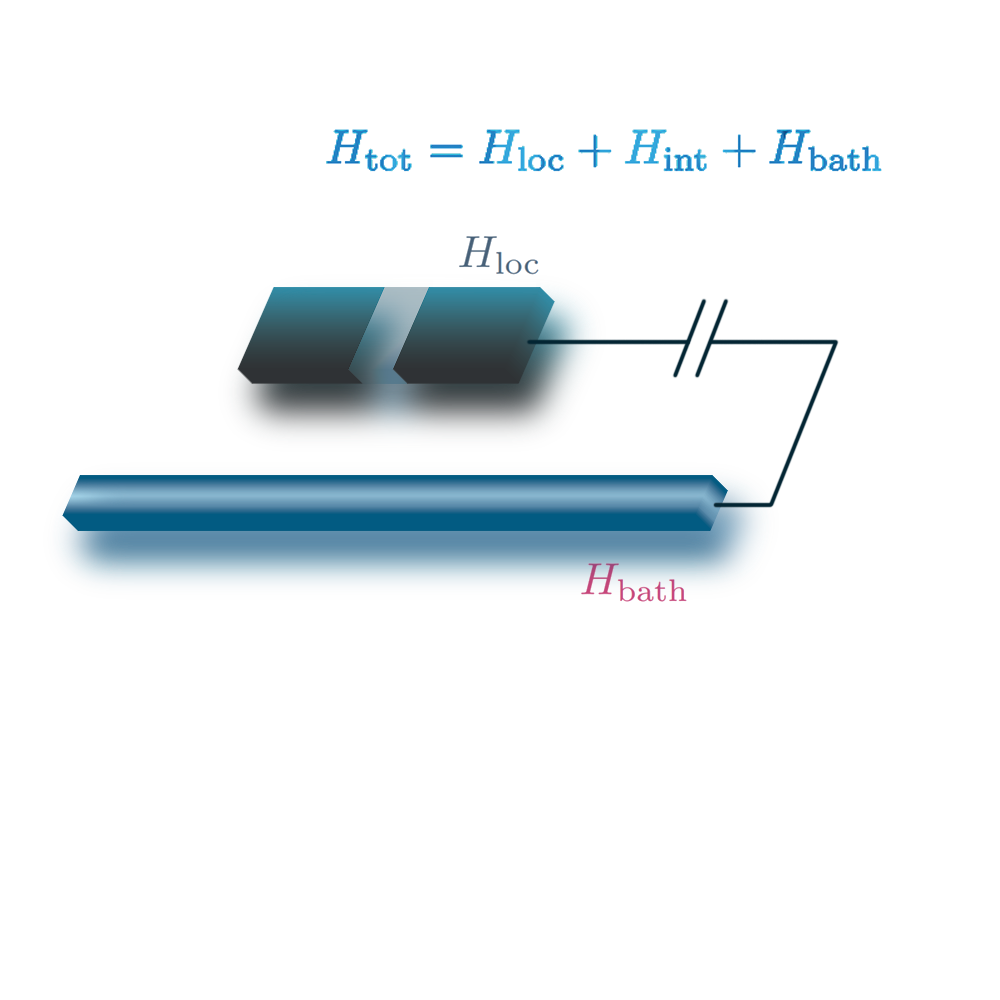
\includegraphics[width=10cm]{TexFigure/Junction_RE.png}}
  \caption{Brief Image of Resistivity shunted Josephson junction}
  \label{fig:RSJJ}
\end{figure}

\begin{figure}[htbp]
  \centerline{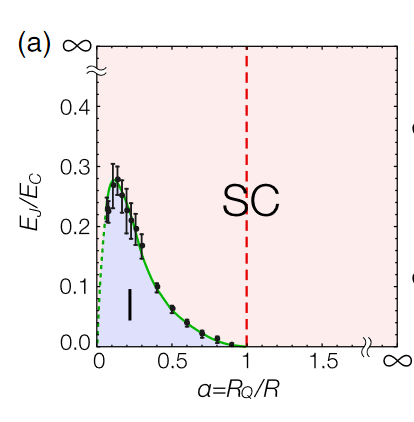
\includegraphics[width=6cm]{TexFigure/kps_INT_exp.PNG}}
  \caption{Zero temperature phase diagram with reentrant phase transition[2]}
  \label{fig:reentrant}
\end{figure}
\end{spacing}
\pagebreak
\section{Theoretical method}
\begin{spacing}{1.5}
\subsection{Circuit model}
\subsubsection*{Hamiltonian of resistivity shunted Josephson junction}
  \begin{figure}[htbp]
    \centerline{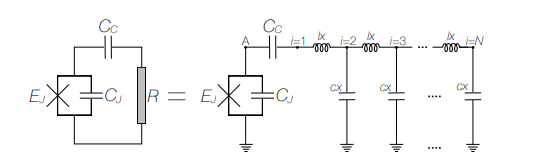
\includegraphics[width=12cm]{TexFigure/circuit_supp_ashida.PNG}}
    \caption{ Picture of resistivity shunted Josephson junction connected with exterior transmission line.[18]}
  \end{figure} 
We introduce the impurity model for the resistivity shunted Josephson junction (RSJJ) circuit . 
Specific Hamiltonians and physical parameters are based on the [2]. 
The circuit is composed of a single Josephson junction connected to the transmission line, 
which acts as the resistance of the total circuit system. 
Each component of the circuit is mapped onto each composition of the total Hamiltonian. 
The given circuit Hamiltonian form is represented as follows : 
\begin{flalign}
  \begin{split}
	  H_{\text{sys}} = (E_c\hat{N^2}-E_J\cos{\phi}) \otimes I -\hat{N} \otimes \sum_{0<k\leq K}\hbar g_k(\hat{b}_k^\dagger + \hat{b}_k) + I \otimes \sum_{0<k\leq K}\hbar\omega_k\hat{b_k}^\dagger\hat{b_k}~,
	  \label{eqn:H_RSJJ}
\end{split}
\end{flalign}
where $\hat{N}=i\partial/\partial\phi$ is the charge operator, $\hat{b}_k$ ($\hat{b}^\dagger_k$) is the bosonic annihilation (creation) operator of $k$-th mode, coupled to the charge of JJ of coupling energy scale $\hbar g_k$

Equation~\ref{eqn:H_RSJJ} can be divided into three parts:
\begin{flalign}
  \begin{split}
	  H_{\text{sys}} = H_{\text{loc}}+H_{\text{int}}+H_{\text{bath}}~,
\end{split}
\end{flalign}
each of which represents the local JJ, the bath bosons, and coupling between them;
\begin{flalign}
  \begin{split}
H_{\text{loc}} &=E_C\hat{N}^2 - E_J \cos{\phi} \\ H_{\text{bath}} &= \sum_{0<k\leq K} \hbar \omega_k \hat{b}^\dagger_k \hat{b}_k \\ H_{\text{int}} &= -\hat{N}\sum_{0<k\leq K} \hbar g_k (\hat{b}^\dagger_k + \hat{b}_k)
\end{split}
\end{flalign}
The detailed description of basic symbols is summarized in Table.~\ref{tab:H}. 
\begin{table}[htbp]
  \centering
  \renewcommand{\arraystretch}{1.2}
  \begin{tabular}{@{}ccc@{}}
  \toprule
  \textbf{Symbols} & \textbf{Formula} & \textbf{Physical quantities} \\ 
  \midrule
  $\phi$ & & Phase of Josephson junction \\ 
  $\hat{N}$ & $-i\frac{\partial}{\partial \phi}$ & Charge operator \\ 
  $\omega_k$ & $vk =\frac{vm\pi}{L}$ & Bath frequency \\ 
  $\hat{b_k}^\dagger,\hat{b_k}$ & & Bosonic creation, annihilation operator \\
  $R_Q$ & $\frac{h}{4e^2}$ & Quantum resistance of junction \\
  $R$ & & Resistance of bath \\
  $E_C$ & $\frac{(2e)^2}{2C_J}$ & Josephson junction charging energy \\ 
  $E_J$ & & Josephson coupling energy \\ 
  $g_k$ & $\sqrt{\frac{2\pi v}{\alpha L} \frac{\omega_k}{1+(\frac{\nu \omega_k}{W})^2}}$ & Coupling with bath in mode $k$ \\ 
  $\nu$ & $\frac{\pi}{\alpha \epsilon_C}$ & \\
  $\epsilon_C$ & $\frac{E_C}{\hbar W}$ & \\
  \bottomrule
  \end{tabular}
  \caption{Basic symbols used for describing Hamiltonian.}
  \label{tab:H}
  \end{table}

  Both in the local JJ and bosonic bath, degrees of freedoms satisfies the fundamental commutation relation: the phase of JJ and its conjugate charge operator in the local Hamiltonian, and annihillation and creation operators for the bath Hamiltonian.
  \begin{align}
	  [\phi,\hat{N}]&=i\hbar~,\nonumber\\
	  [\hat{b}_k,\hat{b}^\dagger_{k'}]&=\delta_{kk'}~.
	  \label{<+label+>}
  \end{align}
  The coupling between the JJ and the $k$-th mode boson is denoted by $g_k$, and $\alpha =\frac{R_Q}{R}$ controls the global coupling strength for all bosonic modes.
  On the other hand, the competition between the Josephson coupling $E_J$ and the charge energy scale $E_C$ is controlled by $\gamma = \frac{E_J}{E_C}$ in the local part. 
  $\alpha$ and $\gamma$ will be our basic control parameters.
  We’ve set $E_C$ as an energy unit.
\subsubsection*{$H_{\text{loc}}$ in Josephson phase basis}
To adjust the expansion method to the RSJJ Hamiltonian model, We represent the local system Hamiltonian in matrix formulation using the basis of Josephson wave function. 
We adopt the macroscopic point of view to observe the superconducting effect expected in our junction system. 
The free-particle wavefunction in the $2\pi$-periodic JJ phase ($\phi$) space can be written in the exponential form: 
\begin{flalign}
  \begin{split}
	  \ket{\psi_{JJ}} = \sum_{-\infty}^{\infty} c_m\frac{e^{im\phi}}{\sqrt{2\pi}}~,
\end{split}
\end{flalign}
where, $e^{im\phi}/\sqrt{2\pi}$ constitutes the complete basis with wavenumber $m$.
In trigonometric form,
\begin{flalign}
  \begin{split}
	  \ket{\psi_{JJ}}=\frac{a_0}{\sqrt{2\pi}} + \frac{1}{\sqrt{\pi}}\sum_{m=1}^\infty (a_m\cos{m\phi} +b_m\sin{m\phi})~.
\end{split}
\end{flalign}
Since the local Hamiltonian doesn't mix the even and odd sectors, one can safely write down the even and odd eigenvectors separately:
\begin{align}
	\ket{\text{even}_k}=\frac{a^{(k)}_0}{\sqrt{2\pi}} + \sum_{n=1}\frac{a^{(k)}_n}{\sqrt{\pi}}\cos{n\phi}~,\\
	\ket{\text{odd}_k} = \sum_{m=1}\frac{b_m^{(k)}}{\sqrt{\pi}}\sin{m\phi}~.
	\label{<+label+>}
\end{align}
Here, $k$ is the eigenstate index.
%Here, $k$ is the eigenstate index, that is, the energy state of the even function basis split by external perturbation in the k-th excited state. In the same way, the eigenvector written in the form of an odd function is as follows: 

%And its matrix form is : 
%\begin{flalign}
%  \begin{split}
%\ket{\text{even}_k}=\begin{pmatrix} \alpha_0 \\ \alpha_1\\ \vdots \\\alpha_m\end{pmatrix}\quad, \quad \ket{\text{odd}_k}=\begin{pmatrix} \beta_1 \\ \beta_2\\ \vdots \\\beta_m\end{pmatrix}
%\end{split}
%\end{flalign}
Considering the differential form of local system Hamiltonian in the trigonometric basis, 
\begin{flalign}
  \begin{split}
H_{\text{loc}} = -\frac{\partial^2}{\partial \phi^2} - \gamma\cos{\phi}
\end{split}
\end{flalign}
the Hamiltonian can be written as follows.
%\begin{flalign}
%  \begin{split}
%&H_{\text{loc}}\ket{\psi_{JJ}} = H_{\text{loc}}(\ket{\text{even}_k}+\ket{\text{odd}_k}) \\ \text{ } 
%\\ &\bigg(-\frac{\partial^2}{\partial \phi^2} - \gamma\cos{\phi}\bigg)\bigg(\sum_{m=0}^\infty a_m\cos{m\phi} +\sum_{n=1}^\infty b_n\sin{n\phi}\bigg) 
%\\&= -\sum_{m=0}^\infty (m^2a_m\cos{m\phi}+\gamma\cos{\phi}\cos{m\phi})-\sum_{n=1}^\infty (n^2b_n\sin{n\phi}+\gamma\cos{\phi}\sin{n\phi})
%\end{split}
%\end{flalign}
%In matrix representation,
\begin{align}
H_{\text{loc even}} &= \begin{pmatrix}
0 & -\frac{\gamma}{\sqrt{2}} & 0 & \cdots \\
-\frac{\gamma}{\sqrt{2}} & 1 & -\frac{\gamma}{2} & 0 & \cdots \\ &  \\
0 & -\frac{\gamma}{2} & 4 &  \\
\vdots &  &  & \ddots 
\end{pmatrix}
\qquad (m = 0,1,2, \dots)~,\\
H_{\text{loc odd}} &= \begin{pmatrix}
1 & -\frac{\gamma}{2} & 0 & \cdots \\
-\frac{\gamma}{2} & 4 & -\frac{\gamma}{2} & 0 & \cdots \\ &  \\
0 & -\frac{\gamma}{2} & 9 &  \\
\vdots &  &  & \ddots 
\end{pmatrix}
\qquad (m = 1,2, \dots)~.
	\label{eqn:Hloc}
\end{align}

One can numerially diagonalize Eq.~\ref{eqn:Hloc}.
And using the fact that the difference between the energy levels becomes larger as $m$ increases, we truncate the local Hilbert space for computationally managable subsets of low-lying states.

%To study how system changes depends on coupling parameters and finite temperature conditions, we measure the total RSJJ Hamiltonian under local system basis engaged from diagonalization of the $H_{\text{loc even}}$ and $H_{\text{loc odd}}$ . 
\subsubsection*{Matrix form of $\hat{N}$ in local eigen basis}
%The charge operator $\hat{N}$ pursues polarization operator in our expansion model, endows coupling effect between local system and bath system. Exploiting local basis from previous procedure, We can write $\hat{N}$ in aspect of local system view. [bullshit\dots]
\subsubsection*{3-level case}
Now, we can span the charge operator in eigenvectors of $H_{\text{loc even}}$ and $H_{\text{loc odd}}$. In 2-level case, we can use total lowest three states as basis vector,
\begin{flalign}
  \begin{split}
	  &\ket{\text{gs}}=\frac{a^{(0)}_0}{\sqrt{2\pi}} + \sum_{n=1}\frac{a^{(0)}_n}{\sqrt{\pi}}\cos{n\phi} = \frac{a_0}{\sqrt{2\pi}} + \frac{a_1}{{\sqrt{\pi}}}\cos{\phi} + \frac{a_2}{\sqrt{\pi}} \cos{2\phi} +\cdots~,\\
&\ket{\text{1st}} = \sum_{m=1}\frac{b^{(1)}_m}{\sqrt{\pi}}\sin{m\phi} = \frac{b_1}{{\sqrt{\pi}}}\sin{\phi} +  \frac{b_2}{\sqrt{\pi}} \sin{2\phi}+\cdots~,\\
&\ket{\text{2nd}}=\frac{a^{(1)}_0}{\sqrt{2\pi}} + \sum_{n=1}\frac{a^{(1)}_n}{\sqrt{\pi}}\cos{n\phi}= \frac{a'_0}{\sqrt{2\pi}} + \frac{a'_1}{{\sqrt{\pi}}}\cos{\phi} + \frac{a'_2}{\sqrt{\pi}} \cos{2\phi} +\cdots~.
\end{split}
\end{flalign}
Here we note the upper indices with round brace to indicate the energy excitation of local system. Then matrix form of $\hat{N}$ becomes :
\begin{flalign}
  \begin{split}
\hat{N} &= \begin{pmatrix}
\bra{\text{gs}}-i\frac{\partial}{\partial\phi}\ket{\text{gs}} & \bra{\text{gs}}-i\frac{\partial}{\partial\phi}\ket{\text{1st}} & \bra{\text{gs}}-i\frac{\partial}{\partial\phi}\ket{\text{2nd}} \\
\bra{\text{1st}}-i\frac{\partial}{\partial\phi}\ket{\text{gs}} &  \bra{\text{1st}}-i\frac{\partial}{\partial\phi}\ket{\text{1st}} & \bra{\text{1st}}-i\frac{\partial}{\partial\phi}\ket{\text{2nd}} \\ 
\bra{\text{2nd}}-i\frac{\partial}{\partial\phi}\ket{\text{gs}} & \bra{\text{2nd}}-i\frac{\partial}{\partial\phi}\ket{\text{1st}} & \bra{\text{2nd}}-i\frac{\partial}{\partial\phi}\ket{\text{2nd}}
\end{pmatrix}~, \\ \quad \\ 
&=i\begin{pmatrix}
0 & \sum_{n=1}na^{(0)}_n b^{(1)}_n & 0\\
-\sum_{n=1}na^{(0)}_n b^{(1)}_n &  0 & -\sum_{n=1}na^{(1)}_n b^{(1)}_n \\ 
0 & \sum_{n=1}na^{(1)}_n b^{(1)}_n & 0
\end{pmatrix}~.
\end{split}
\end{flalign}
\subsubsection*{Multilevel case}
For the higher-level case, one can easily generalize the matrix expression of $\hat{N}$~.
Now based on the above discussion, the extended form of charge operator in higher dimension is :
\begin{flalign}
  \begin{split}
\hat{N} &= \begin{pmatrix}
\bra{\text{gs}}-i\frac{\partial}{\partial\phi}\ket{\text{gs}} & \bra{\text{gs}}-i\frac{\partial}{\partial\phi}\ket{\text{1st}} & \cdots \\
\bra{\text{1st}}-i\frac{\partial}{\partial\phi}\ket{\text{gs}} &  \ddots & \vdots \\ 
\vdots & \cdots & \bra{\text{nth}}-i\frac{\partial}{\partial\phi}\ket{\text{nth}}
\end{pmatrix} \\ \quad \\ 
&=i\begin{pmatrix}
0 & \sum_{n=1}na^{(0)}_n b^{(1)}_n & \cdots \\
-\sum_{n=1}na^{(0)}_n b^{(1)}_n &  \ddots & \ \\ & &-\sum_{n=1}na^{(n-1)}_n b^{(n)}_n \\ 
\vdots & \sum_{n=1}na^{(n-1)}_n b^{(n)}_n & 
\end{pmatrix}
\end{split}
\end{flalign}
$\\$
In this case, the maximum dimension of $\hat{N}$  is $2n+1$ .
\pagebreak
\subsubsection*{Matrix Form of $\hat{\cos\phi}$}
The physical observable $\hat{\cos\phi}$ represents the phase coherence of the currents flowing at both ends of the Josephson junction. 
If the junction exhibits superconducting properties, the value of $\hat{\cos\phi}$ will be greater than 0, 
while it will be close to 0 if it exhibits insulating properties.
The expectation of $\hat{\cos\phi}$ can be calculated in following formula:
\begin{flalign}
  \begin{split}
  \langle \cos\phi\rangle = \frac{\text{Tr}[\hat{\cos\phi}e^{\beta H}]}{\text{Tr}[e^{-\beta H}]}
\end{split}
\end{flalign}
\subsubsection*{3-level case}
Since we aim to understand the system from the perspective of which represents the Josephson junction with three energy levels, 
we intend to expand order parameter $\cos \phi$ in simliar procedure with calculating $\hat{N}$ matrix. Adopting the form of fourier basis 
in the case of 3-level in the representing $\hat{N}$ matrix, $\cos\phi$ can be rewritten as a matrix operator, and 
\begin{flalign}
  \begin{split}
\hat{\cos{\phi}} = \begin{pmatrix}
\bra{\text{gs}}\cos{\phi} \ket{\text{gs}} & \bra{\text{gs}}\cos{\phi}\ket{\text{1st}} & \bra{\text{gs}}\cos{\phi}\ket{\text{2nd}}  \\
\bra{\text{1st}}\cos{\phi}\ket{\text{gs}} & \bra{\text{1st}}\cos{\phi}\ket{\text{1st}} & \bra{\text{1st}}\cos{\phi}\ket{\text{2nd}}  \\
\bra{\text{2nd}}\cos{\phi}\ket{\text{gs}} & \bra{\text{2nd}}\cos{\phi}\ket{\text{1st}} & \bra{\text{2nd}}\cos{\phi}\ket{\text{2nd}} \\
\end{pmatrix} 
\end{split}
\end{flalign}
When obtaining eigenvectors for the 3-level truncated 3*3 $H_{\text{loc}}$ matrix, the matrix form of $\cos\phi$ is expressed as follows.
\begin{flalign}
  \begin{split}
\hat{\cos{\phi}} = \begin{pmatrix}
\frac{2}{\sqrt{2}}a_0a_1 + a_1a_2 & 0 & \frac{1}{\sqrt{2}}(a_1a'_0 + a_0a'_1) + \frac{1}{2}(a_1a'_2 + a_2a'_1)  \\
0 & b_1b_2 & 0  \\
\frac{1}{\sqrt{2}}(a_1a'_0 + a_0a'_1) + \frac{1}{2}(a_1a'_2 + a_2a'_1) & 0 & \frac{2}{\sqrt{2}}a'_0a'_1 + a'_1a'_2 \\
\end{pmatrix} 
\end{split}
\end{flalign}
$\\$
\subsubsection*{Multilevel case}
When including more than 3 levels, expressing the order parameter in matrix form for the Hamiltonian $H_{\text{loc}}$ involves the following steps.
First, the calculation of the even function form of the order parameter $\cos \phi$ is as follows:
\begin{flalign}
  \begin{split}
\cos{\phi} \ket{\text{even}_k} = \frac{a^{(k)}_0}{\sqrt{2\pi}}\cos{\phi} + \sum_{n=1}\frac{a^{(k)}}{\sqrt{\pi}}\cos{\phi}\cos{n\phi}
\end{split}
\end{flalign}
And final inner product result is:
\begin{flalign}
  \begin{split}
\bra{\text{even}_l}\cos{\phi} \ket{\text{even}_k} = \int^{2\pi}_0\bigg(\frac{a^{(m)}_0}{\sqrt{2\pi}} + \sum_{m=1}\frac{a^{(m)}}{\sqrt{\pi}}\cos{m\phi}\bigg)\bigg(\frac{a^{(n)}_0}{\sqrt{2\pi}}\cos{\phi} + \sum_{n=1}\frac{a^{(n)}}{\sqrt{\pi}}\cos{\phi}\cos{n\phi}\bigg)
\end{split}
\end{flalign}
The calculation for the odd function form is as follows:
\begin{flalign}
  \begin{split}
\ket{\text{odd}}=\sum_{n=1} \frac{b_n^{(k)}}{\sqrt{\pi}}\sin{n\phi} \quad , \quad
\cos{\phi}\ket{\text{odd}}=\sum_{n=1}\frac{b_n^{(k)}}{\sqrt{\pi}}\cos{\phi}\sin{n\phi}
\end{split}
\end{flalign}
Similar with the case of even state eigenvector, innerproduct result is:
\begin{flalign}
  \begin{split}
    &\bra{\text{odd}_l}\cos{\phi} \ket{\text{odd}_k} = \sum_{n,m=1}\int^{2\pi}_0 d\phi \bigg(\frac{b_n^{(k)}b_m^{(l)}}{\pi}\cos{\phi}\sin{n\phi}\sin{m\phi}\bigg) \\
    &=    \left\{
        \begin{array}{ll}
            \text{if k} < \text{l : }  \qquad \sum^N_{n=1} \bigg(\frac{\hat{b}^{(k)}_n\hat{b}^{(l)}_{n-1}}{2} + \frac{\hat{b}^{(k)}_n\hat{b}^{(l)}_{n+1}}{2}\bigg)\\
            \text{if k } > \text{l : }  \qquad \sum^N_{n=1} \bigg(\frac{\hat{b}^{(k)}_{n-1}\hat{b}^{(l)}_{n}}{2} + \frac{\hat{b}^{(k)}_{n+1}\hat{b}^{(l)}_{n}}{2}\bigg)
        \end{array}
        \right.
\end{split}
      \end{flalign}
Therefore, when the entire $\cos{\phi}$ is expressed in matrix form, it takes the following form:
\begin{flalign}
  \begin{split}
    \hat{\cos{\phi}} = \begin{pmatrix}
       \ddots & & \vdots & & \\
      & \bra{\text{even}_k}\cos\phi\ket{\text{even}_k} & 0 & \bra{\text{even}_k}\cos\phi\ket{\text{even}_{k+1}} & \cdots \\
      & 0 & \bra{\text{odd}_k}\cos\phi\ket{\text{odd}_k} & 0 & \bra{\text{odd}_k}\cos\phi\ket{\text{odd}_{k+1}} \\
      & \bra{\text{even}_{k+1}}\cos\phi\ket{\text{even}_k} & 0 & \bra{\text{even}_{k+1}}\cos\phi\ket{\text{even}_{k+1}} & \\
      & & \vdots & &\ddots \\
      \end{pmatrix} 
    \end{split}
    \end{flalign}
\end{spacing}
\pagebreak
\subsection{Diagrammatic method}
\subsubsection*{Field operator and Green's function}
\begin{spacing}{1.5}
In this chapter, we will briefly summarize the theoretical framework of the Green’s function method, 
  and pseudo-particle solvers, such as non-crossing approximation (NCA). 
In quantum many-body theory, the physical system is depicted over the frame of the fermionic(bosonic) 
creation and annihilation operator, and $\hat{a}(\hat{a}^\dagger)$ as an annihilation(creation) operator, 
it satisfies the following commutation relations:
\begin{flalign}
  \begin{split}
[\hat{a_i},\hat{a_j}] &= \{\hat{a_i},\hat{a_j}\} = 0 \\ 
[\hat{a_i}^\dagger,\hat{a_j}^\dagger] &= \{\hat{a_i}^\dagger,\hat{a_j}^\dagger\}=0\\ 
[\hat{a_i},\hat{a_j}^\dagger] = \{\hat{a_i},\hat{a_j}^\dagger\} &= \delta_{ij} = \begin{cases} 1 \quad (i=j)\\  0 \quad (i \neq j)\quad \end{cases}
\end{split}
\end{flalign}
Where the square bracket informs the bosonic case, and its RHS indicates the fermionic case. In the following discussion, we will drop out the lower indices of the field operator, assuming it can indicate any arbitrary quantum states.
If we consider the Hamiltonian system can be split into two parts: for the local system and for interaction, we can write the total Hamiltonian $H$:
\begin{flalign}
  \begin{split}
H = H_0 + H_{\text{int}}
\end{split}
\end{flalign}
Here, $H_0$ is the local(Free) Hamiltonian, $H_{\text{int}}$  is the Hamiltonian for interaction (external potential). To express the dynamics of a given operator, we depict the time dependency of the operator in the interaction picture :
\begin{flalign}
  \begin{split}
\hat{a}(t) = e^{iH_0t}\hat{a}e^{-iH_0t} \\ \hat{a}^\dagger(t) =  e^{-iH_0t}\hat{a}^\dagger e^{iH_0t} 
\end{split}
\end{flalign}
With the above time dependency, we can define the Green’s function as follows :
\begin{flalign}
  \begin{split}
G_0(t,t') = \frac{i}{\hbar}\langle \mathcal{T}\hat{a}^\dagger(t)\hat{a}(t')\rangle = \begin{cases} \frac{i}{\hbar}\langle \hat{a}^\dagger(t)\hat{a}(t')\rangle  \quad (t>t')\\  \pm\frac{i}{\hbar}\langle \hat{a}(t')\hat{a}^\dagger(t)\rangle \quad (t<t')\quad \end{cases}
\end{split}
\end{flalign}
Here, the symbol $\mathcal{T}$ is the time ordering operator. One of the features of Green’s function is that it satisfies the given equation of motion :
\begin{flalign}
  \begin{split}
[i \partial_t-H] &G(t,t')=\delta(t-t') \\
[i \partial_t-H_0]G_0(t,t')&=[i \partial_t-H+H']G_0(t,t')=\delta(t-t')
\end{split}
\end{flalign}
\subsubsection*{Diagrammatic expansion of Green’s function}
In the statistical framework, it is easy to calculate Green’s function in the imaginary time $\tau$ due to the wick rotation of the time axis, which mapped time-dependent system progression into thermal equilibrium problems with temperature dependency.
\begin{flalign}
  \begin{split}
\frac{it}{\hbar}=\tau = \beta = \frac{1}{k_BT}
\end{split}
\end{flalign}
We will use $\hbar=1$ in overall discussion. In this new frame, Green’s function can be rewritten :
\begin{flalign}
  \begin{split}
G_0(\tau,\tau') = \langle\mathcal{T}\hat{a}^\dagger(\tau)\hat{a}(\tau)\rangle\begin{cases} \langle \hat{a}^\dagger(\tau)\hat{a}(\tau')\rangle  \quad (\tau>\tau')\\  \pm \langle \hat{a}(\tau')\hat{a}^\dagger(\tau)\rangle \quad (\tau<\tau')\quad \end{cases}
\end{split}
\end{flalign}
There are particular relationship between real-time Green’s function and imaginary time(temperature dependence) Green’s function, which is :
\begin{flalign}
  \begin{split}
G(t,t')\vert_{t=0} = \pm e^{\beta H} G(t,t')\vert_{t=i\beta}
\end{split}
\end{flalign}
These temperature dependence Green’s function is often called as Matsubara Green’s function. 
Single Green’s function corresponding with one specific imaginary time interval can be represented in a diagrammatic way, 
which is the very basic formulation of the diagrammatic method. We can draw a line from $\tau'$  to $\tau$,
\begin{figure}[htbp]
  \centerline{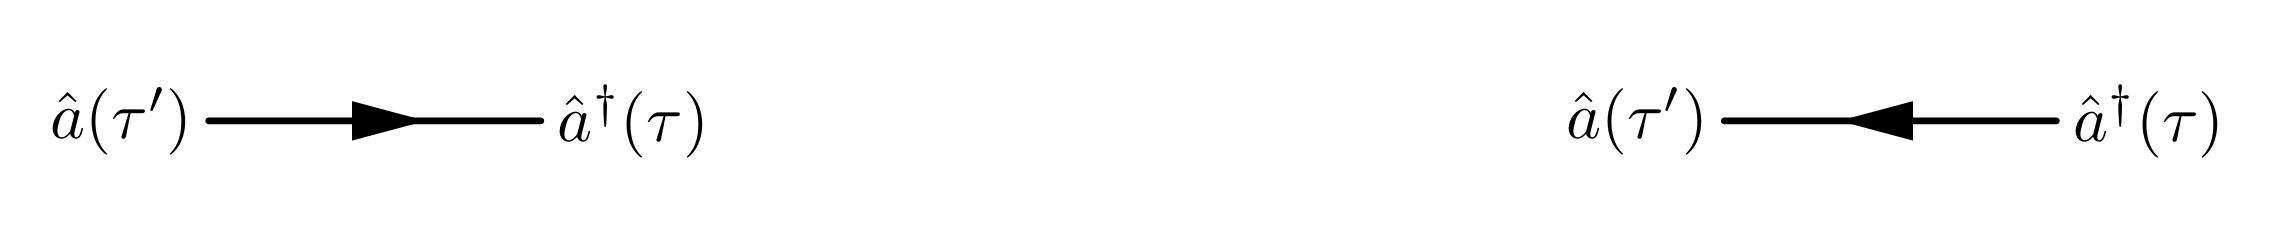
\includegraphics[width=15cm]{TexFigure/Diagram_arrow.PNG}}
  \caption{Diagram of single Green's function. The direction of arrow corresponds with the direction of time flow.}
\end{figure}
\\
In equilibrium statistical mechanics, the expectation value of the physical observable is characterized by the partition function that satisfies the given restricted energy condition in phase space. Based on these concepts, on the grand canonical ensemble, the statistical structure of counting Green’s function becomes :  
\begin{flalign}
  \begin{split}
G_0(\tau,\tau') = \frac{\text{Tr}[e^{-\beta H_0} \hat{a}^\dagger(\tau)\hat{a}(\tau')]}{\text{Tr}[e^{-\beta H_0}]} =\frac{\text{Tr}[e^{-\beta H_0} e^{iH_0 \tau} \hat{a}^\dagger e^{-H_0 (\tau-\tau')}\hat{a}e^{-iH_0 \tau'}]}{\text{Tr}[e^{-\beta H_0}]}
\end{split}
\end{flalign}
This is the very basic form of Green’s function in imaginary time corresponding to the diagram structure. Similar case with the creation and annihilation operator, the time dependency of external potential term Hamiltonian : 
\begin{flalign}
  \begin{split}
H'(\tau) = e^{H_0\tau}He^{-H_0\tau}
\end{split}
\end{flalign}
If we consider the effect of interaction, we can adopt full Green’s function includes the interaction operator $U(\tau)$,
\begin{flalign}
  \begin{split}
G(\tau,\tau') = \frac{\text{Tr}[e^{-\beta H_0} U(\beta)\hat{a}^\dagger(\tau)\hat{a}(\tau')]}{\text{Tr}[e^{-\beta H_0}U(\beta)]} =\frac{\text{Tr}[e^{-\beta H} U(\tau) \hat{a}^\dagger U(\tau'-\tau)\hat{a}U(\tau')]}{\text{Tr}[e^{-\beta H}]} 
\end{split}
\end{flalign}
where interaction operator is : 
\begin{flalign}
  \begin{split}
U(\tau) = \mathcal{T}e^{-\int^\tau_0 d\tau' H_{\text{int}}(\tau')}
\end{split}
\end{flalign}
In the imaginary time interval $[\tau,0]$ , full Green’s function in the expectation form can be represented , 
\begin{flalign}
  \begin{split}
G(\tau,0) = \frac{\text{Tr}[e^{-\beta H_0} U(\beta)\hat{a}^\dagger(\tau)\hat{a}]}{\text{Tr}[e^{-\beta H_0}U(\beta)]} = \frac{\langle U(\beta)\hat{a}^\dagger(\tau)\hat{a}\rangle_0}{\langle U(\beta)\rangle_0}
\end{split}
\end{flalign}
The under index 0 of angled bracket indicates its expectation value was calculated in $H_{\text{loc}}$ frame. 
If the interaction hamiltonian is in the form of multiplication of pair of 
annihilation-creation operator $\hat{a}^\dagger$ and $\hat{a}$ , 
we can adjust Wick’s theorem to expand the each of the expectation value in 
denominator and numerator into a multiplication of Green’s functions in each time interval.
A brief discussion for Wick's theorem will be introduced in the Appendix.
\pagebreak
\subsubsection*{Diagrammatic expansion in strong coupling case}
The Hamiltonian system can be divided into three parts as a general case of the time-dependent impurity model with a bosonic bath:
\begin{flalign}
  \begin{split}
    H_{sys} = H_{loc}+H_{int}+H_{bath}
  \end{split}
\end{flalign}
In the second quantized form, This can be rewritten:
\begin{flalign}
  \begin{split}
H(t) = H_{loc}(t) + \underbrace{\sum_n \epsilon_n \hat{b}^\dagger_n}_\text{bath} \hat{b}_n + \underbrace{\sum_{m,n} [V_{m,n}(t) c_m^\dagger b_n + \text{H.c.}]}_\text{interaction}
\end{split}
\end{flalign}
The operator $\hat{b} (\hat{b}^\dagger)$  indicates bosonic annihilation(creation) operator, $\hat{c}(\hat{c}^\dagger)$ is fermionic annihilation(creation) operator. 
Based on this structure, the expansion method was constructed. 
Continue, from the Hamiltonian, the action of the full system can be written into :
\begin{flalign}
  \begin{split}
S = \int^\beta_0 d\tau H_{\text{loc}}(\tau) + \int^\beta_0 d\tau d\tau' P(\tau)\mathcal{W}(\tau-\tau')P(\tau')
\end{split}
\end{flalign}
Here, $H_{\text{loc}}$is the Hamiltonian of the local system, indicating the impurity that we want to focus on. The terms $P$ and $\mathcal{W}$ correspond with the Hermitian operator and the interaction term.
While considering the interaction process, the term $\mathcal{W}$ includes the scalar factor to represent the effect of the bosonic bath. 
With similar procedure with the diagram expansion, We can calculate the expectation value of observable using the partition function $Z$,
\begin{flalign}
  \begin{split}
Z=\text{tr}\bigg[T_{\tau}e^{-S}\bigg]
\end{split}
\end{flalign}
This result takes the form of Dyson's equation in quantum mechanics, which can be represented in the diagram structure. If we define full $\mathcal{G}$ as :
\begin{flalign}
  \begin{split}
\mathcal{G} = \langle\psi_a(\tau)\psi_b^\dagger(\tau')\rangle = \text{Tr}[e^{\beta H}\psi_a(\tau)\psi_b^\dagger(\tau')]
\end{split}
\end{flalign}
Then the diagram of the Dyson equation turns out to Figure.4.
\begin{figure}[H]
  \centerline{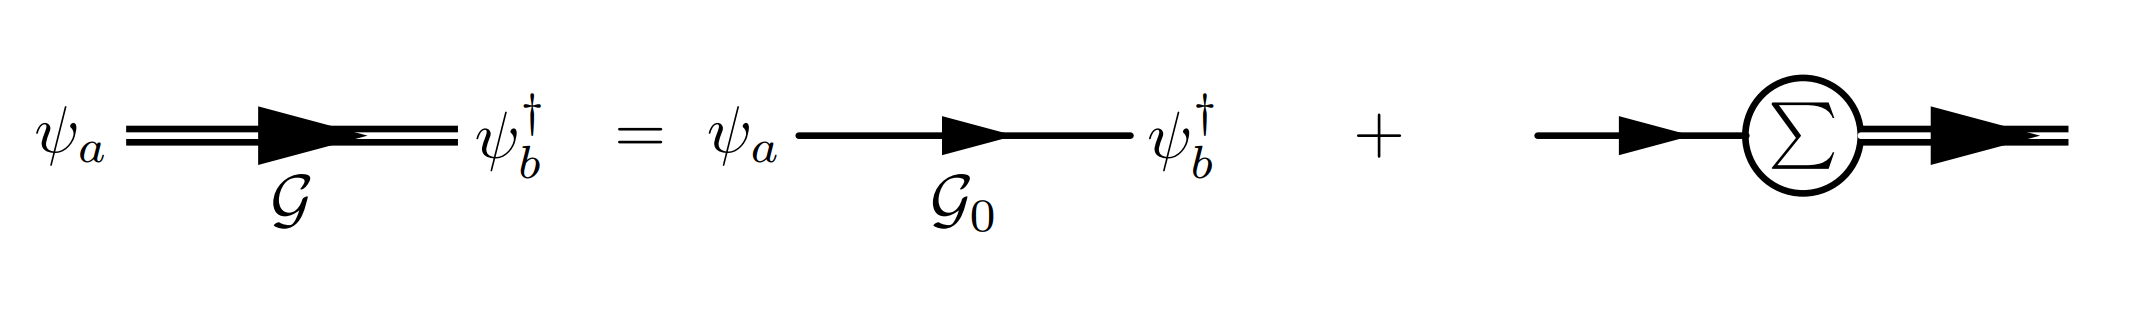
\includegraphics[width=13cm]{TexFigure/Dyson_eq.PNG}}
  \caption{Diagram for Dyson equation with self energy}
\end{figure}
This form of equation satisfies the integral-differential form, agrees with the equation of motion of in the quantum mechanical 
aspect.
\begin{flalign}
  \begin{split}
[-\partial_{\tau}-H_{\text{loc}}+\lambda]\mathcal{G}(\tau)-\int^\tau_0 d\tau_1\Sigma(\tau-\tau_1)\mathcal{G}(\tau_1) = 0 \quad, \quad(\tau>0)
\end{split}
\end{flalign}
\subsubsection*{Evaluation of correlation function}
The Correlation function for green’s function is defined as follows:
\begin{flalign}
  \begin{split}
\chi_{sp}(\tau) &=\frac{1}{Z}\text{Tr}[e^{-S}P(\tau)P(0)] \\
  \end{split}
\end{flalign}
where $S$ is a action of system. Corresponding topological diagram is:
\begin{figure}[hbtp]
  \centerline{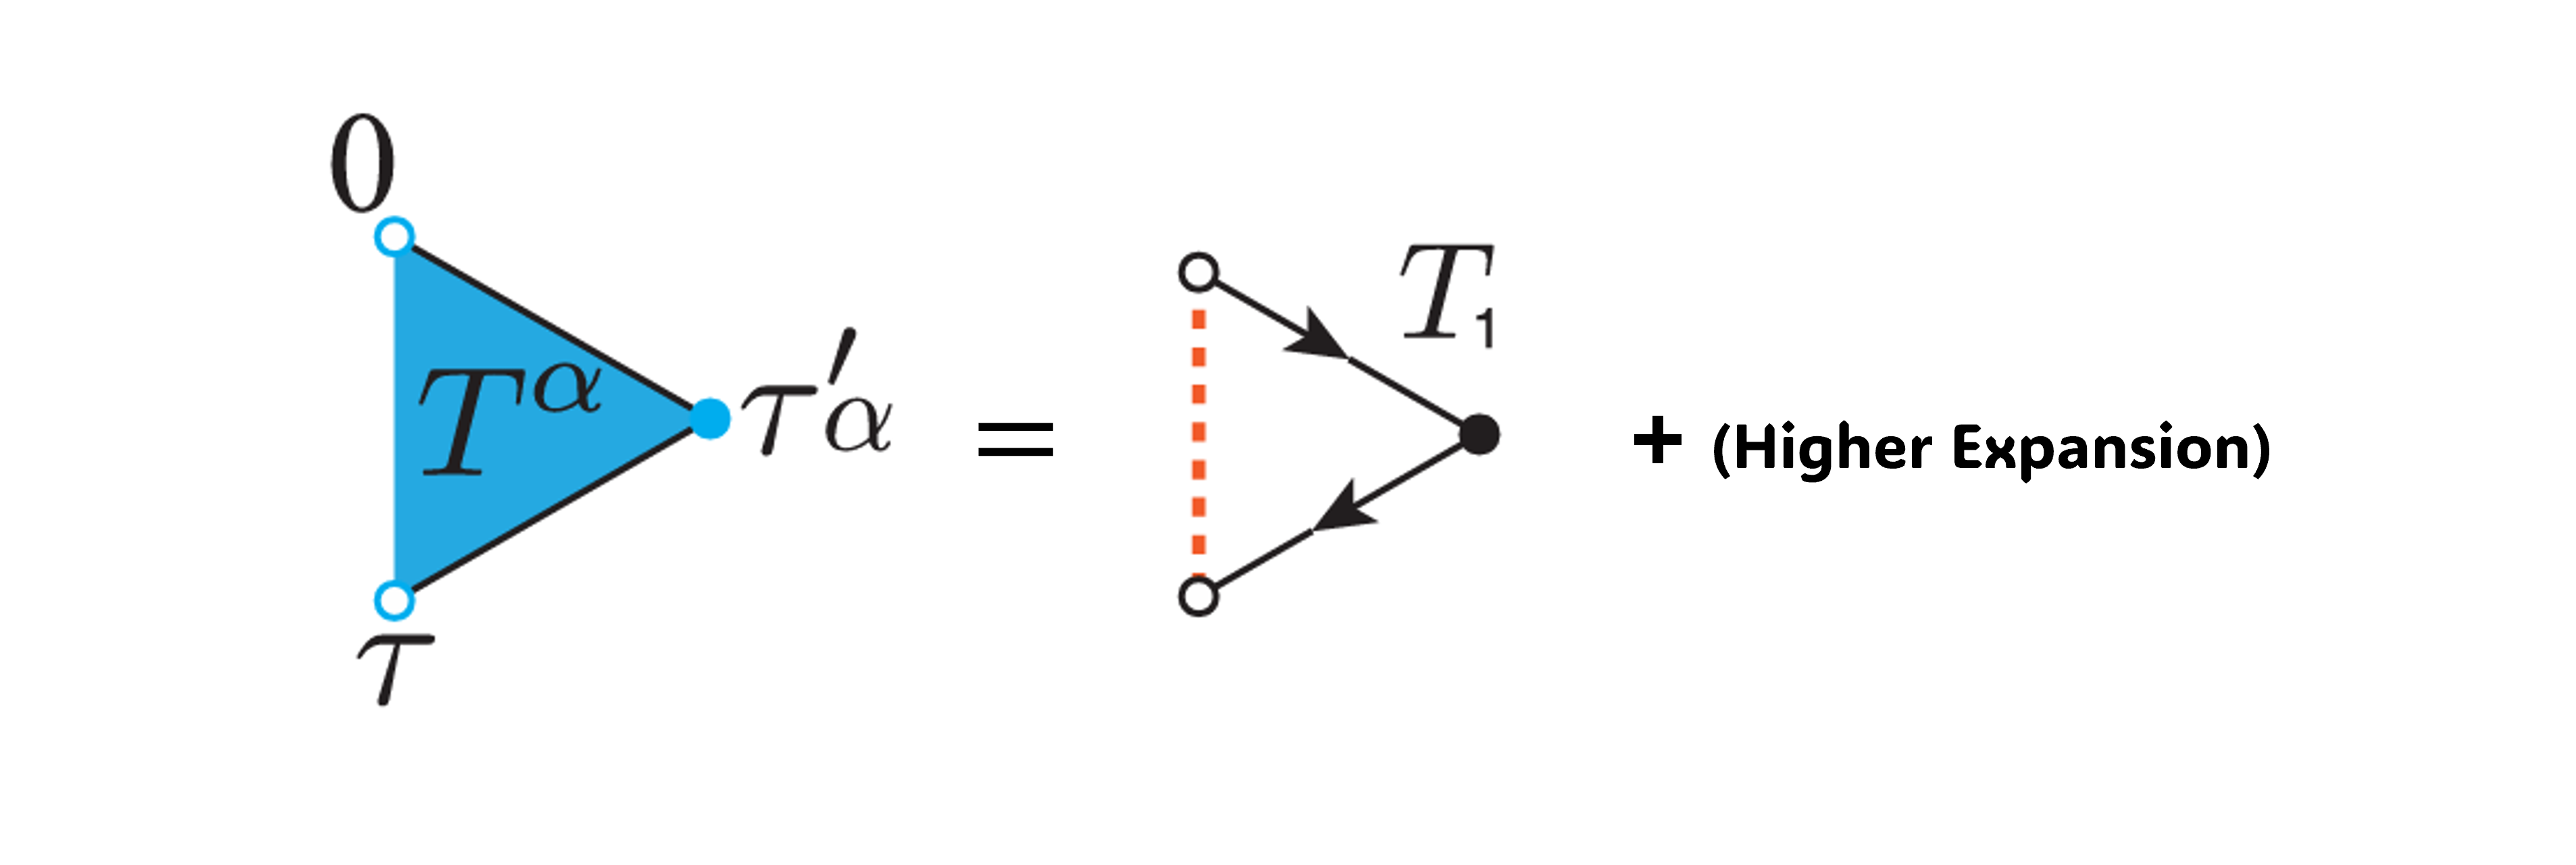
\includegraphics[width=12cm]{TexFigure/Tmat_diagram.png}}
  \centerline{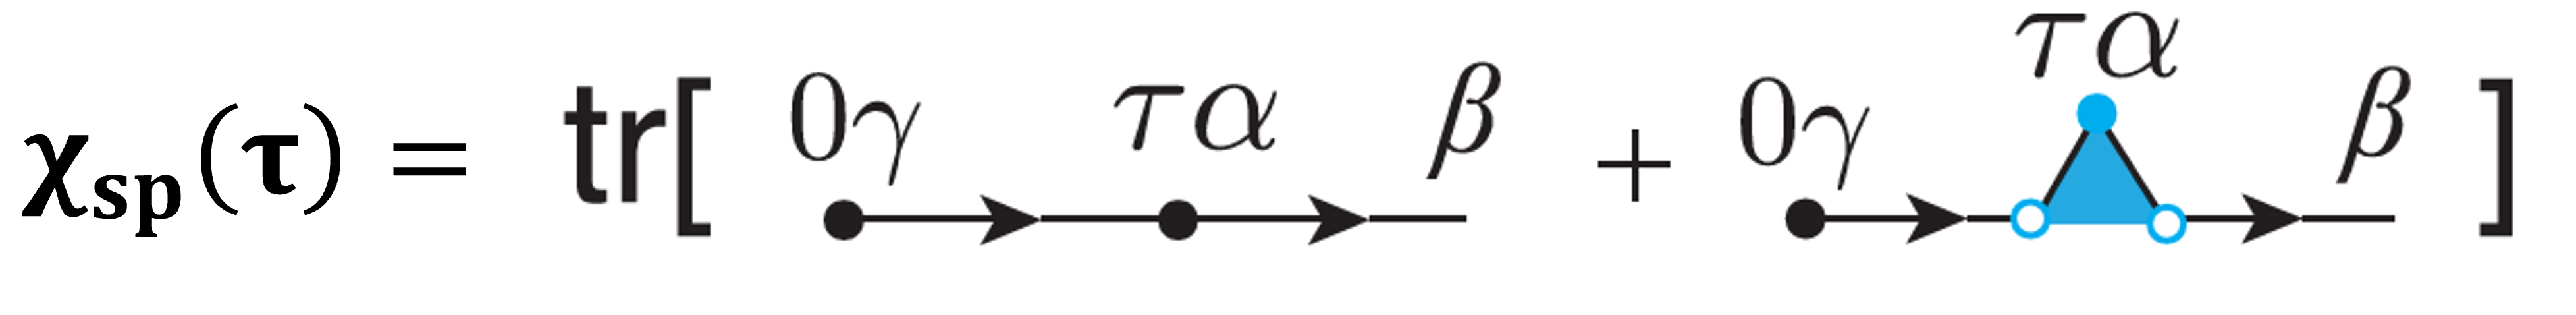
\includegraphics[width=12cm]{TexFigure/Chi_with_Tmat.png}}
  \caption{Specific diagram for T matrix[4].}
\end{figure}

\newpage
\subsection{Applying to circuit hamiltonian model}
\begin{spacing}{1.5}
  In this section, we will introduce how we adjust the expansion method to our circuit model. The basic notation
  and mathematical structure follow the reference[4,5].
In our study, we consider that the total system turns out to be a thermal equilibrium state thus methodology using Matsubara’s method is available. To begin, we assume that each operator from RSJJ Hamiltonian mapped toward the general impurity model:
\begin{table}[htbp]
  \centering
  \renewcommand{\arraystretch}{1.2}
  \begin{tabular}{@{}ccc@{}}
  \toprule
  \textbf{Hamiltonian} &\textbf{RSJJ} & \textbf{Impurity} \\ 
  \midrule
  $H_{\text{bath}}$ &   $\sum_k \hbar\omega_k\hat{b}_k^\dagger\hat{b}_k$ & $\sum_n\epsilon_n\hat{b}_n^\dagger\hat{b}_n$ \\
  $H_\text{int}$ & $\sum_k g_k \hat{N}(\hat{b}^\dagger_k + \hat{b_k})$ & $\sum_{m,n} [V_{m,n}(t) c_m^\dagger b_n + \text{H.c.}]$ 
\end{tabular}
\caption{Comparison with term from Circuit hamiltonian and impurity solver}
\end{table}
More specifically, each parameter has corresponding relations,
\begin{flalign}
  \begin{split}
\hbar\omega_k &\rightarrow \epsilon_n \\
g_k &\rightarrow V_{m,n}\\ 
\hat{N} &\rightarrow \hat{c}^\dagger_m (\hat{c}_m) \\ 
\hat{b}_k^\dagger (\hat{b}_k) &\rightarrow \hat{b}_n^\dagger (\hat{b}_n)
\end{split}
\end{flalign}
Using the relations, we can calculate the system’s partition function as we dealt with in the eqn(2.44).
Notice that instead of the fermion operator $\hat{c}^\dagger (\hat{c})$, 
the operator $\hat{N}$ is written in the vector space spanned through the eigenstates of the Josephson junction. 
\subsubsection*{Calculation of bosonic action}
To focus our attention on the local system where we are interested, we calculate the expectation value of partition function in the aspects of the bath, which eliminates the effects of the bath by evaluating the system dynamics in bath points of view:
\begin{flalign}
  \begin{split}
Z &= Z_{\text{bath}}\text{Tr}_{JJ}\bigg[\frac{\text{Tr}[e^{-\beta H_\text{bath}}U_{sys}(\tau)]}{\text{Tr}[e^{-\beta H_\text{bath}}]}\bigg] \\ 
&= Z_\text{bath}\text{Tr}_{\text{JJ}}[\langle \mathcal{T}_\tau e^{-\int^\beta_0 H_\text{loc}(\tau) + H_\text{bath} + H_\text{int}}\rangle_\text{b}]
\end{split}
\end{flalign}
Here the term $\text{JJ}$ means tracing out the effect of local system, in our case, Josephson junction system, and term is tracing out the effect of bosonic effect, which is $\bra{n_b}\mathcal{O}\ket{n_b}$, $n_b$ is number operator for bosonic field operator, $\mathcal{O}$ is physical quantity to calculate.
To expand the interaction term, we can rewrite the equation into :
\begin{flalign}
  \begin{split}
Z=Z_{\text{bath}}\text{Tr}_{JJ}[\langle \mathcal{T}_\tau e^{-\int^\beta_0 H_\text{loc}(\tau) + H_\text{bath}}\sum_l Z_l\rangle_\text{b}]
\end{split}
\end{flalign}
Here, $l$ corresponds with the number of highest order of perturbative expansion. The derivation of Term $Z_k$ begins from
\begin{flalign}
  \begin{split}
 \mathcal{T}_\tau e^{-\int^\beta_0 H_{\text{int}}(\tau)} \approx 1 -\int^{\beta}_0 H_{\text{int}}(\tau) d\tau +\frac{1}{2} \int^\beta_0 H_{\text{int}}(\tau_1)H_{\text{int}}(\tau_2)d\tau_1 d\tau_2 + \cdots
\end{split}
\end{flalign}
And 
\begin{flalign}
  \begin{split}
Z_l =&\sum_{k_1 \cdots k_l}\sum_{k'_1 \cdots k'_l} g_{k_1}g_{k'_1}g_{k_2}g_{k'_2} \cdots g_{k_l}g_{k'_l} \int^\beta_0 d\tau_1 \int^\beta_{\tau_1}d\tau_2 \cdots\int^\beta_{\tau_{{l-1}}}d\tau_{l} \int^\beta_0 d\tau_1 \int^\beta_{\tau'_1}d\tau'_2 \cdots\int^\beta_{\tau'_{{l-1}}}d\tau'_{l} 
\\ & \times \hat{N}(\tau_1)\hat{b}^\dagger_{k_1}(\tau_1)\hat{N}(\tau'_1)\hat{b}_{k'_1}(\tau'_1)  \hat{N}(\tau_2)\hat{b}^\dagger_{k_2}(\tau_2)\hat{N}(\tau'_2)\hat{b}_{k'_2}(\tau'_2) \cdots \hat{N}(\tau_{l})\hat{b}^\dagger_{k_l}(\tau_{l})\hat{N}(\tau'_{l})\hat{b}_{k'_l}(\tau'_{l})
\end{split}
\end{flalign}
Here the lower index $k_i$ indicates the oscillation mode of the ith harmonic oscillator from bath that is represented as a pair of bosonic creation and annihilation operators. The number $\frac{1}{k_l !}$ was eliminated due to considering all permutations during ordering time.
Notice that, \textit{1.} $k_i =k'_j$ \textit{ for all }(i,j)  , 
\textit{2. } $\hat{N}$ \textit{ and  } $\hat{b}_k^\dagger(\hat{b_k})$\textit{  are defined on different vector space , thus   }
$[\hat{N},\hat{b}^\dagger (\hat{b})] = 0$ , we can adjust $Z_l$ as follows :
\begin{flalign}
  \begin{split}
Z_l = &\sum_{k_1 \cdots k_l} (g_{k_1}g_{k_2} \cdots g_{k_l})^2\int^\beta_0 d\tau_1 \int^\beta_{\tau_1}d\tau_2 \cdots\int^\beta_{\tau_{k_{l-1}}}d\tau_{k_l} \int^\beta_0 d\tau_1 \int^\beta_{\tau'_1}d\tau'_2 \cdots\int^\beta_{\tau'_{k_{l-1}}}d\tau_{k_l} \\ 
&\times \hat{N}(\tau_1)\hat{b}^\dagger_{k_1}(\tau_1)\hat{b}_{k_1}(\tau'_1)\hat{N}(\tau'_1)  \hat{N}(\tau_2)\hat{b}^\dagger_{k_2}(\tau_2)\hat{b}_{k_2}(\tau'_2)\hat{N}(\tau'_2) 
\cdots \hat{N}(\tau_{k_l})\hat{b}^\dagger_{k_l}(\tau_{k_l})\hat{b}_{k_l}(\tau'_{k_l})\hat{N}(\tau'_{k_l})
\end{split}
\end{flalign}
To calculate the effect of bath, the form of the equation turns out:  
\begin{flalign}
  \begin{split}
\langle & \mathcal{T}_\tau e^{-\int^\beta_0 H_\text{loc}(\tau) + H_\text{bath}}\sum_l Z_l\rangle_\text{b} \\ 
&= \mathcal{T}_\tau e^{-\int^\beta_0 H_{loc}}\langle \mathcal{T}_\tau e^{-\int^\beta_0  H_\text{bath}}\sum_l Z_l\rangle_\text{b} \\ 
&=\mathcal{T}_\tau e^{-\int^\beta_0 H_{loc}}\langle \mathcal{T}_\tau e^{-\int^\beta_0  H_\text{bath}}\sum_l \text{(bosonic terms)}\rangle_\text{b} \\ 
\times \int^\beta_0 d\tau_1 \int^\beta_{\tau_1}d\tau_2 \cdots\int^\beta_{\tau_{k_{l-1}}} & d\tau_{k_l} \int^\beta_0 d\tau_1 \int^\beta_{\tau'_1}d\tau'_2 \cdots\int^\beta_{\tau'_{k_{l-1}}}d\tau_{k_l}
 \hat{N}(\tau_1)\hat{N}(\tau'_1)  \hat{N}(\tau_2)\hat{N}(\tau'_2) 
\cdots \hat{N}(\tau_{k_l})\hat{N}(\tau'_{k_l})
\end{split}
\end{flalign}
Here, each bosonic term contains a calculation of form $\langle \hat{b}^\dagger_{k_1}(\tau_1)\hat{b}_{k_1}(\tau'_1)\hat{b}^\dagger_{k_2}(\tau_2)\hat{b}_{k_2}(\tau'_2)\cdots\hat{b}^\dagger_{k_l}(\tau_l)\hat{b}_{k_l}(\tau'_l)\rangle_\text{b}$, where Wick’s theorem is available. 
Before applying Wick’s theorem to a given equation, notice that there are natural restrictions due to the independence of harmonic oscillators in the bath which do not interact with each others, leading to only one available property for contraction,
\begin{flalign}
  \begin{split}
\langle \hat{b}^\dagger_{k_1}(\tau_1)\hat{b}_{k_1}(\tau'_1)\hat{b}^\dagger_{k_2}(\tau_2)\hat{b}_{k_2}(\tau'_2)&\cdots\hat{b}^\dagger_{k_l}(\tau_l)\hat{b}_{k_l} (\tau'_l)\rangle_\text{b} \\
 = &\langle \hat{b}^\dagger_{k_1}(\tau_1)\hat{b}_{k_1}(\tau'_1)\rangle_\text{b} \langle\hat{b}^\dagger_{k_2}(\tau_2)\hat{b}_{k_2}(\tau'_2)\rangle_\text{b}\cdots\langle\hat{b}^\dagger_{k_l}(\tau_l)\hat{b}_{k_l} (\tau'_l)\rangle_\text{b} 
 \\ & +\langle \hat{b}_{k_1}(\tau'_1)\hat{b}^\dagger_{k_1}(\tau_1)\rangle_\text{b} \langle\hat{b}_{k_2}(\tau'_2)\hat{b}^\dagger_{k_2}(\tau_2)\rangle_\text{b}\cdots\langle\hat{b}_{k_l}(\tau'_l)\hat{b}^\dagger_{k_l} (\tau_l)\rangle_\text{b}
\end{split}
\end{flalign}
Which is full bosonic term turn out to sum of multiplication of single bosonic Green’s function.
It is known that when the ensemble Hamiltonian, aimed at observing a certain physical quantity, takes the form of a harmonic oscillator, 
it can be expressed as $\hat{a}^\dagger(\tau) = e^{E\tau} , \hat{a}(\tau) = e^{-E\tau}\hat{a}$  where $E$ is a eigenvalue of Hamiltonian.[7] 
Using this formula, each single Green’s function can be calculated as:
\begin{flalign}
  \begin{split}
\langle e^{-\omega_k \tau}\hat{b}^\dagger_k e^{-\omega_k \tau'}\hat{b}_k\rangle_\text{b} &= \langle e^{\omega_p (\tau-\tau')}\hat{b}^\dagger_k\hat{b}_k\rangle_\text{b} = e^{\omega_k \tau}n_\text{B}(\omega_k) \qquad (\tau>\tau') \\
\langle e^{-\omega_k \tau}\hat{b}_k e^{-\omega_k \tau'}\hat{b}^\dagger_k\rangle_\text{b} = \langle e^{\omega_p (\tau-\tau')}\hat{b}_k\hat{b}^\dagger_k\rangle_\text{b} &= \langle e^{\omega_p (\tau-\tau')}(1+\hat{b}_k^\dagger\hat{b}_k\rangle_\text{b} = e^{\omega_k (\tau-\tau')}(1+n_\text{B}(\omega_k)) \qquad (\tau<\tau')
  \end{split}
\end{flalign}
By multiplying the corresponding coupling parameter $g_k^2$ in mode $k$ , the full equation becomes :
\begin{flalign}
  \begin{split}
\langle \mathcal{T}_\tau e^{-\int^\beta_0  H_\text{bath}} Z_l\rangle_\text{b} =g^2_{k_1}\big(e^{\omega_{k_1}(\tau_1-\tau'_1)}(\theta(\tau_1-\tau'_1)n_\text{B}(\omega_{k_1})+\theta(\tau'_1-\tau_1)[1+n_\text{B}(\omega_{k_1})])\big) \\
\times g^2_{k_2}\big(e^{\omega_{k_2}(\tau_2-\tau'_2)}(\theta(\tau_2-\tau'_2)n_\text{B}(\omega_{k_2})+\theta(\tau'_2-\tau_2)[1+n_\text{B}(\omega_{k_2})])\big)\\
\vdots\\
\times g^2_{k_l}\big(e^{\omega_{k_l}(\tau_l-\tau'_l)}(\theta(\tau_l-\tau'_l)n_\text{B}(\omega_{k_l})+\theta(\tau'_l-\tau_l)[1+n_\text{B}(\omega_{k_l}]))\big)
\end{split}
\end{flalign}
In the general approach, the term that corresponds to $\mathcal{W}$  from pseudo-particle solver can be expressed as follows:
\begin{flalign}
  \begin{split}
\mathcal{W}(\tau)=\begin{cases}  \sum_k |g_k|^2 e^{\omega_k \tau}n_{\text{B}}(\omega_k) \qquad (\tau>0) \\ \sum_k |g_k|^2 e^{\omega_k \tau}[1+n_{\text{B}}](\omega_k) \quad (\tau<0) \end{cases}
  \end{split}
\end{flalign}
And instead of notation $\mathcal{\bar{W}}$, we use $V_k(\tau)$  to representing simultaneously for retarded and advanced cases, 
\begin{flalign}
  \begin{split}
V_k(\tau) = e^{-\omega_k\tau}\theta(-\tau)n_B(\omega_k \beta)  + e^{-\omega_k\tau}\theta(\tau)(1+n_B(\omega_k \beta))
\end{split}
\end{flalign}
In which we can rewrite as the form of:
\begin{flalign}
  \begin{split}
V_k(\tau)= e^{-\omega_k\tau} \frac{\cosh{\frac{\omega_k}{2}}}{\sinh{\frac{\omega_k}{2}}}
\end{split}
\end{flalign}
\subsubsection*{Calculation of Propagator}
Now, after calculating the bosonic action, we can calculate the structure of propagator. 
To begin, the result of equation (2.44) after caculating $\bar{\mathcal{W}}$ turns out to :
\begin{flalign}
\begin{split}
Z = Z_{\text{bath}}\text{Tr}_\text{JJ}\big[\mathcal{T}_\tau e^{-\int^\beta_0 d\tau H_{\text{loc}}(\tau)} \langle \mathcal{T}_\tau e^{-\int^\beta_0 d\tau H_{\text{bath}}(\tau)} \sum_lZ_l\rangle_{\text{b}}\big] 
\end{split}
\end{flalign}
Where $Z_l$  is :
\begin{flalign}
\begin{split}
Z_l = \sum_{\mathcal{P}\in S}\sum_{k_1 \cdots k_l} \int  ^\beta_0 d\tau_1 \cdots \int^\beta_0 d\tau_{k_l}\int^\beta_0 d\tau'_1 \cdots \int^\beta_0d\tau'_{k_l} \bar{\mathcal{W}}\hat{N}(\tau_{k_1})\hat{N}(\tau'_{k_1})\hat{N}(\tau_{k_2})\hat{N}(\tau'_{k_2})\cdots \hat{N}(\tau_{k_l})\hat{N}(\tau'_{k_l})
\end{split}
\end{flalign}
Here $\mathcal{P}$ indicates the possible permutation which $\mathcal{P} \in S$  
for $\{S| \text{All possible permutation satisfying condition}\}$.
The trace for Josephson junction turns out to :
\begin{flalign}
  \begin{split}
\text{Tr}_{JJ}\bigg[\sum_l \sum_{\mathcal{P}\in S}\sum_{k_1 \cdots k_l} \int^\beta_0 d\tau_{k_1} \cdots \int^\beta_0 d\tau'_{k_l} \bar{\mathcal{W}}_k \cdot \mathcal{T}_\tau e^{-\int^\beta_0 d\tau H_{loc}(\tau)}\hat{N}(\tau_{k_1})\hat{N}(\tau'_{k_1})\cdots\hat{N}(\tau_{k_l})\hat{N}(\tau'_{k_l})\bigg]
  \end{split}
\end{flalign}
Based upon above form, we can define self-energy the above formula in the different $l$ values.
\begin{flalign}
\begin{split}
l = 1 \quad, \quad \text{Tr}_{JJ}\bigg[\sum_{\mathcal{P} \in S} \sum_{\text{(mode)}} \int^\beta_0 d\tau_{k_1} \int^\beta_0 d\tau'_{k_1} \bar{\mathcal{W}} \cdot \underbrace{\mathcal{T}_\tau e^{-\int^\beta_0 d\tau H_{loc}(\tau)} \hat{N}(\tau_{k_1})\hat{N}(\tau'_{k_1})}\bigg] \\
U(\beta-\tau_{k_1})\cdot \underbrace{\bar{\mathcal{W}}\cdot\hat{N}U(\tau_{k_1}-\tau'_{k_1})\hat{N}U(\tau'_{k_1})}_{=\Sigma^{(1)}}
\end{split}
\end{flalign}
\begin{flalign}
\begin{split}
l = 2 \quad, \quad \text{Tr}_{JJ}\bigg[\sum_{\mathcal{P} \in S} \sum_{\text{(mode)}} \int^\beta_0 d\tau_{k_1} \int^\beta_0 d\tau'_{k_1} \int^\beta_0 d\tau_{k_2} \int^\beta_0 d\tau'_{k_2}\bar{\mathcal{W}} \cdot \underbrace{\mathcal{T}_\tau e^{-\int^\beta_0 d\tau H_{loc}(\tau)} \hat{N}(\tau_{k_1})\hat{N}(\tau'_{k_1})\hat{N}(\tau_{k_2})\hat{N}(\tau'_{k_2})}\bigg] \\
U(\beta-\tau_{k_1})\cdot \underbrace{\bar{\mathcal{W}}\cdot\hat{N}U(\tau_{k_1}-\tau'_{k_1})\hat{N}U(\tau'_{k_1}-\tau_{k_2})\hat{N}U(\tau_{k_2}-\tau'_{k_2})\hat{N}}_{=\Sigma^{(2)}}U(\tau'_{k_2})
\end{split}
\end{flalign}
For instance, if we consider only the first-order self-energy expansion, 
the result coincides with the well-known Non-crossing approximation method. Here, the ordering of the time index dominated through pre-decided $\bar{\mathcal{W}}$. 
In the order $l = 1$, the structure of the diagram corresponds with a Non-crossing approximation. 
And the case $l = 2$, it corresponds with a One-crossing approximation. Getting more diagrams corresponding with a higher-order expansion such as TOA, 
can be achievable by increasing the maximum value of the $l$ index.
\subsubsection*{Calculating correlation function}
After calculating the action in the above section and calculating the remaining terms again for the Josephson junction, 
we can obtain terms of the form of equation (2.60). Through calculating the correlation function as in equation (2.50) using the obtained form, we additionally intro
duced an operator λ1 defined as follows:
\begin{flalign}
\begin{split}
  \lambda_1 = 
  \begin{pmatrix}
    0 & 1 & 0 \\
    1 & 0 & 0 \\
    0 & 0 & 0
  \end{pmatrix}
\end{split}
\end{flalign}
This operator was introduced to investigate the degree of mixing between the ground state and the first excited state among the energy states of the junction. 
By applying operator, the final expression for calculating the correlation function in the RSJJ Hamiltonian model can be written as follows:
\begin{flalign}
  \begin{split}
    \chi_{sp}(\tau) &=\text{Tr}[\mathcal{G}(\beta-\tau)\lambda_1\mathcal{G}(\tau)\lambda_1] \\
                    & + \int\int \text{Tr}[V(\tau_2-\tau_1)\mathcal{G}(\beta-\tau_1)\hat{N}\mathcal{G}(\tau_1-\tau_2)\lambda_1\mathcal{G}(\tau_2 - \tau)\hat{N}\mathcal{G}(\tau)\lambda_1]\\
                    & + \cdots
  \end{split}
\end{flalign}
\pagebreak
\begin{figure}[H]
  \centerline{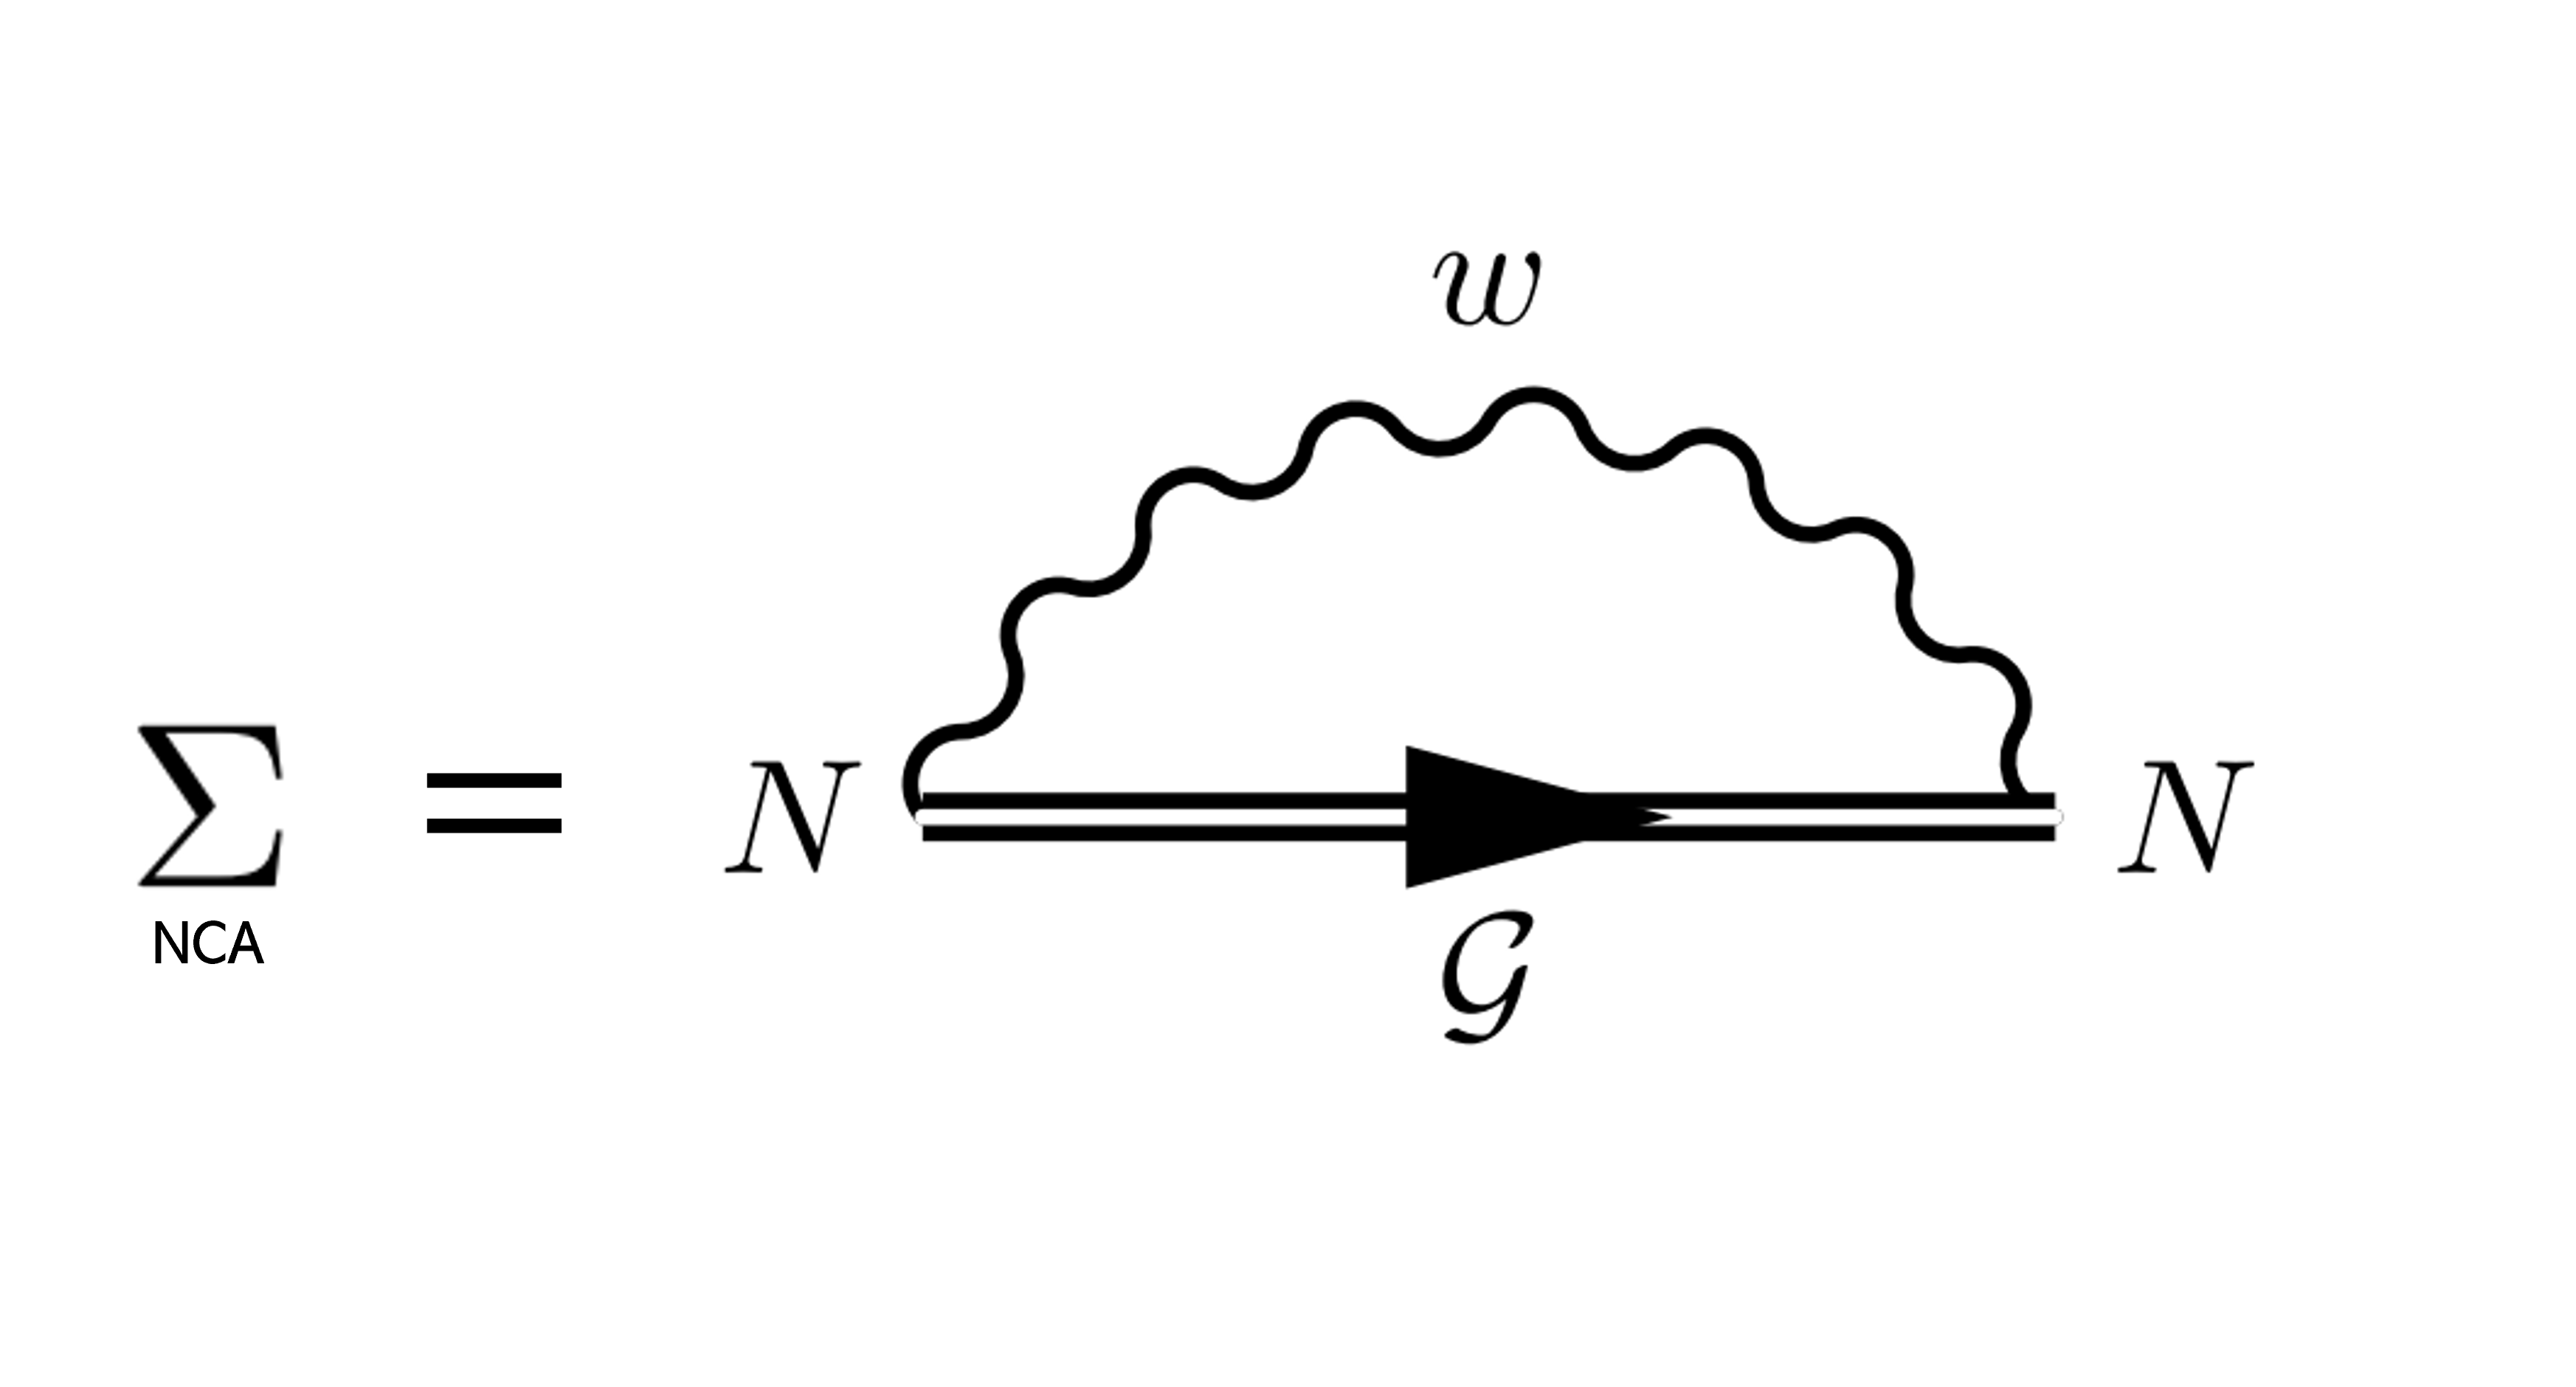
\includegraphics[width=8cm]{TexFigure/NCA_self.PNG}}
  \centerline{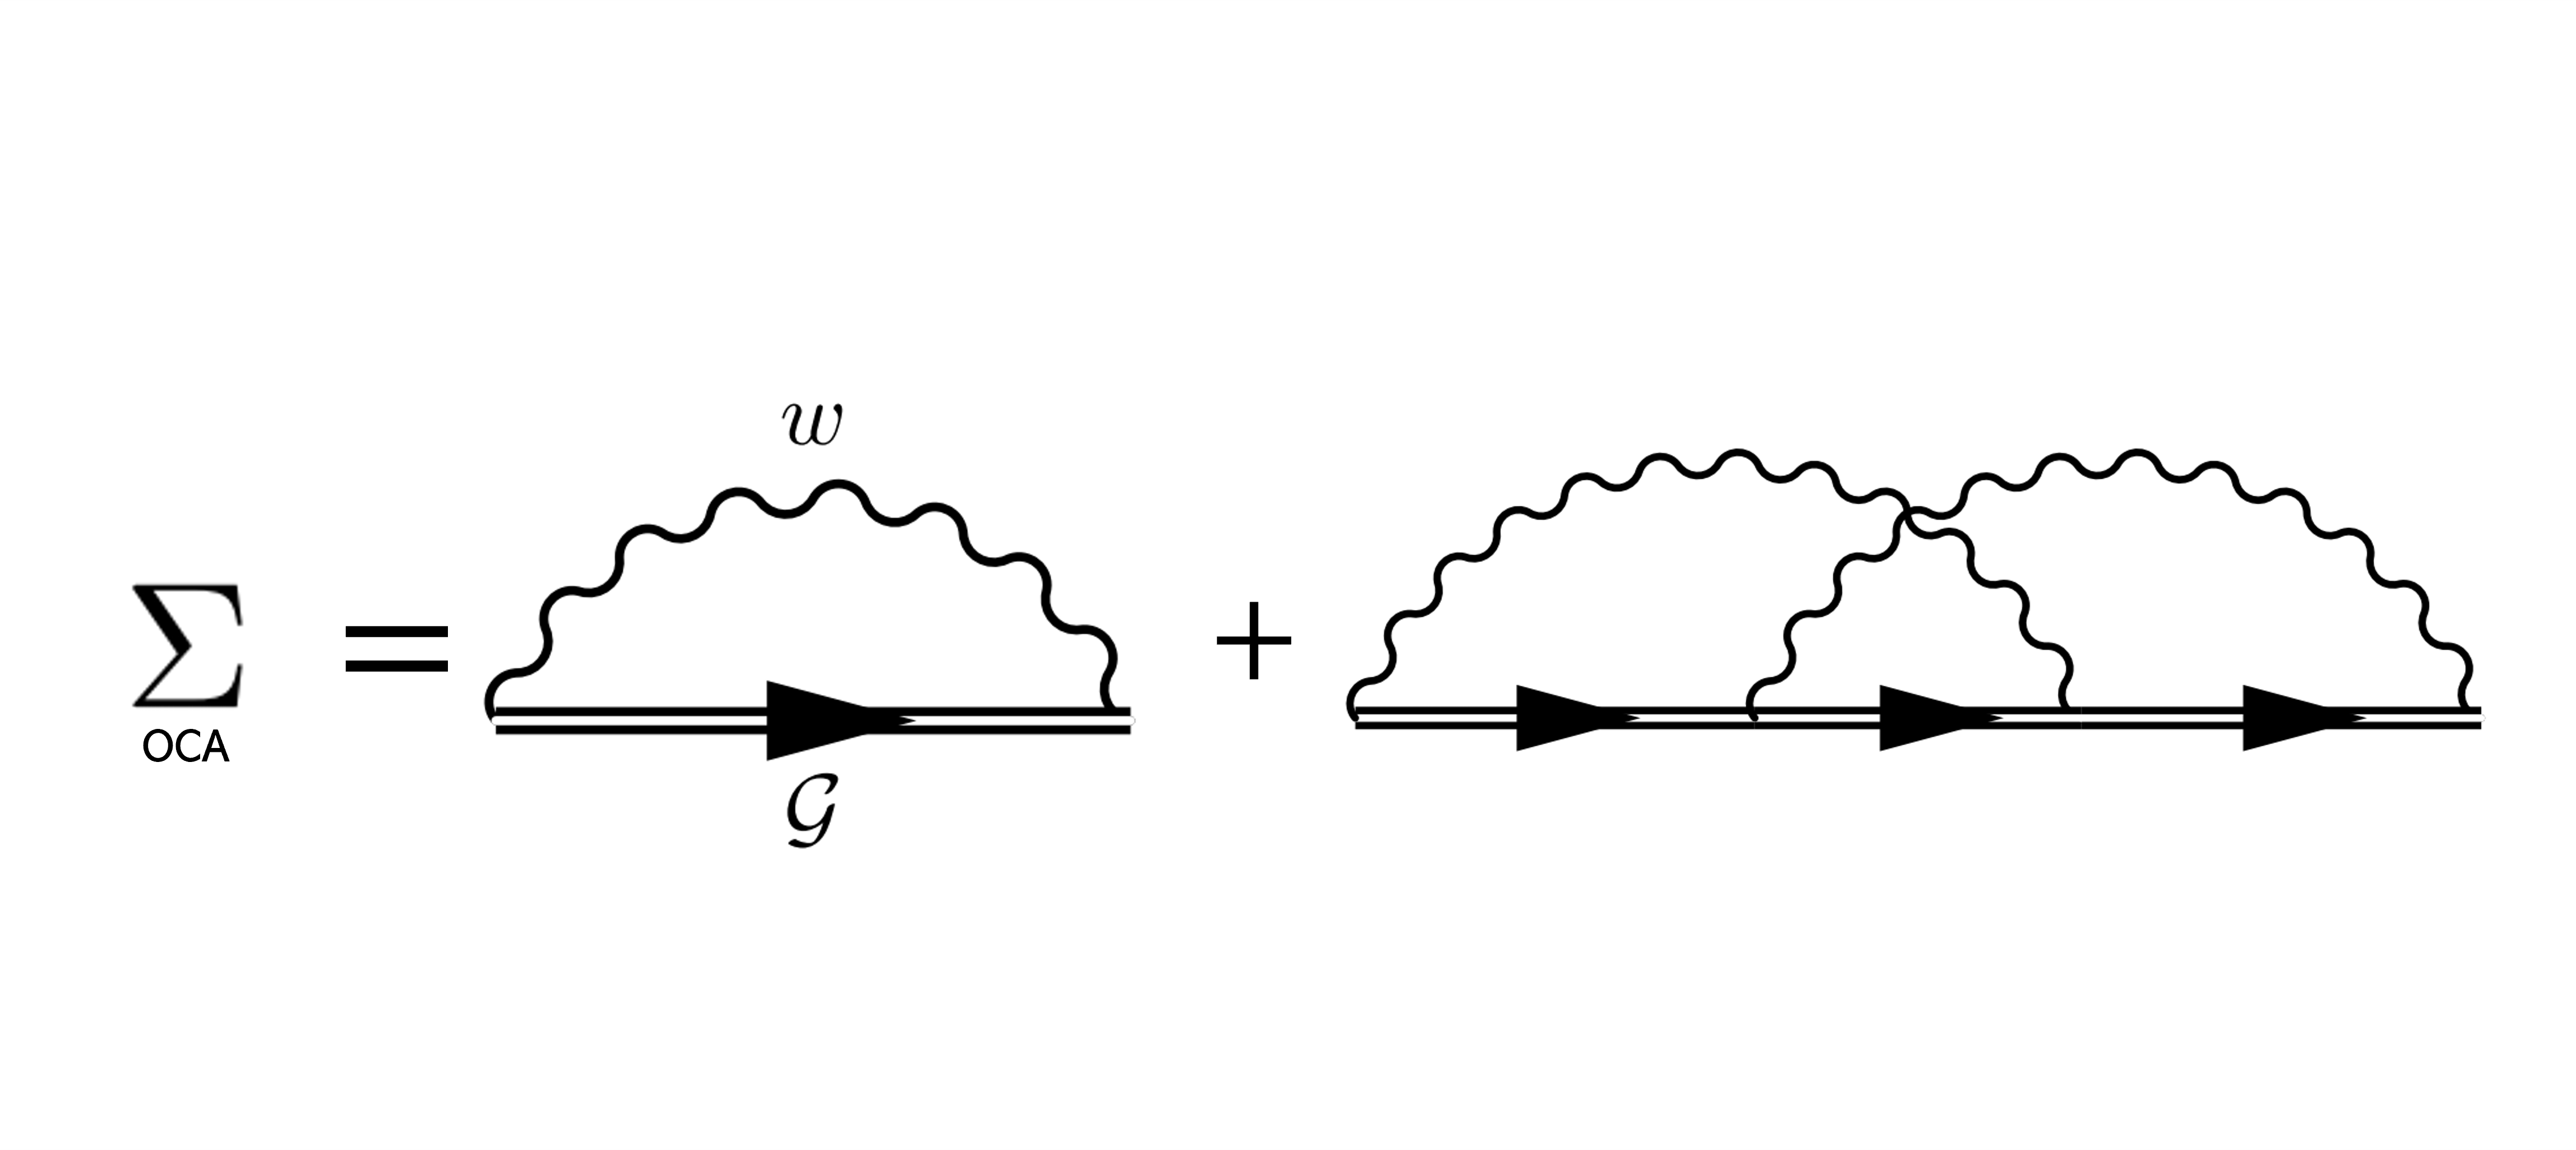
\includegraphics[width=12cm]{TexFigure/OCA_self.PNG}}
  \caption{Self-energy diagram for order of expansion}
\end{figure}
\begin{figure}[H]
  \centerline{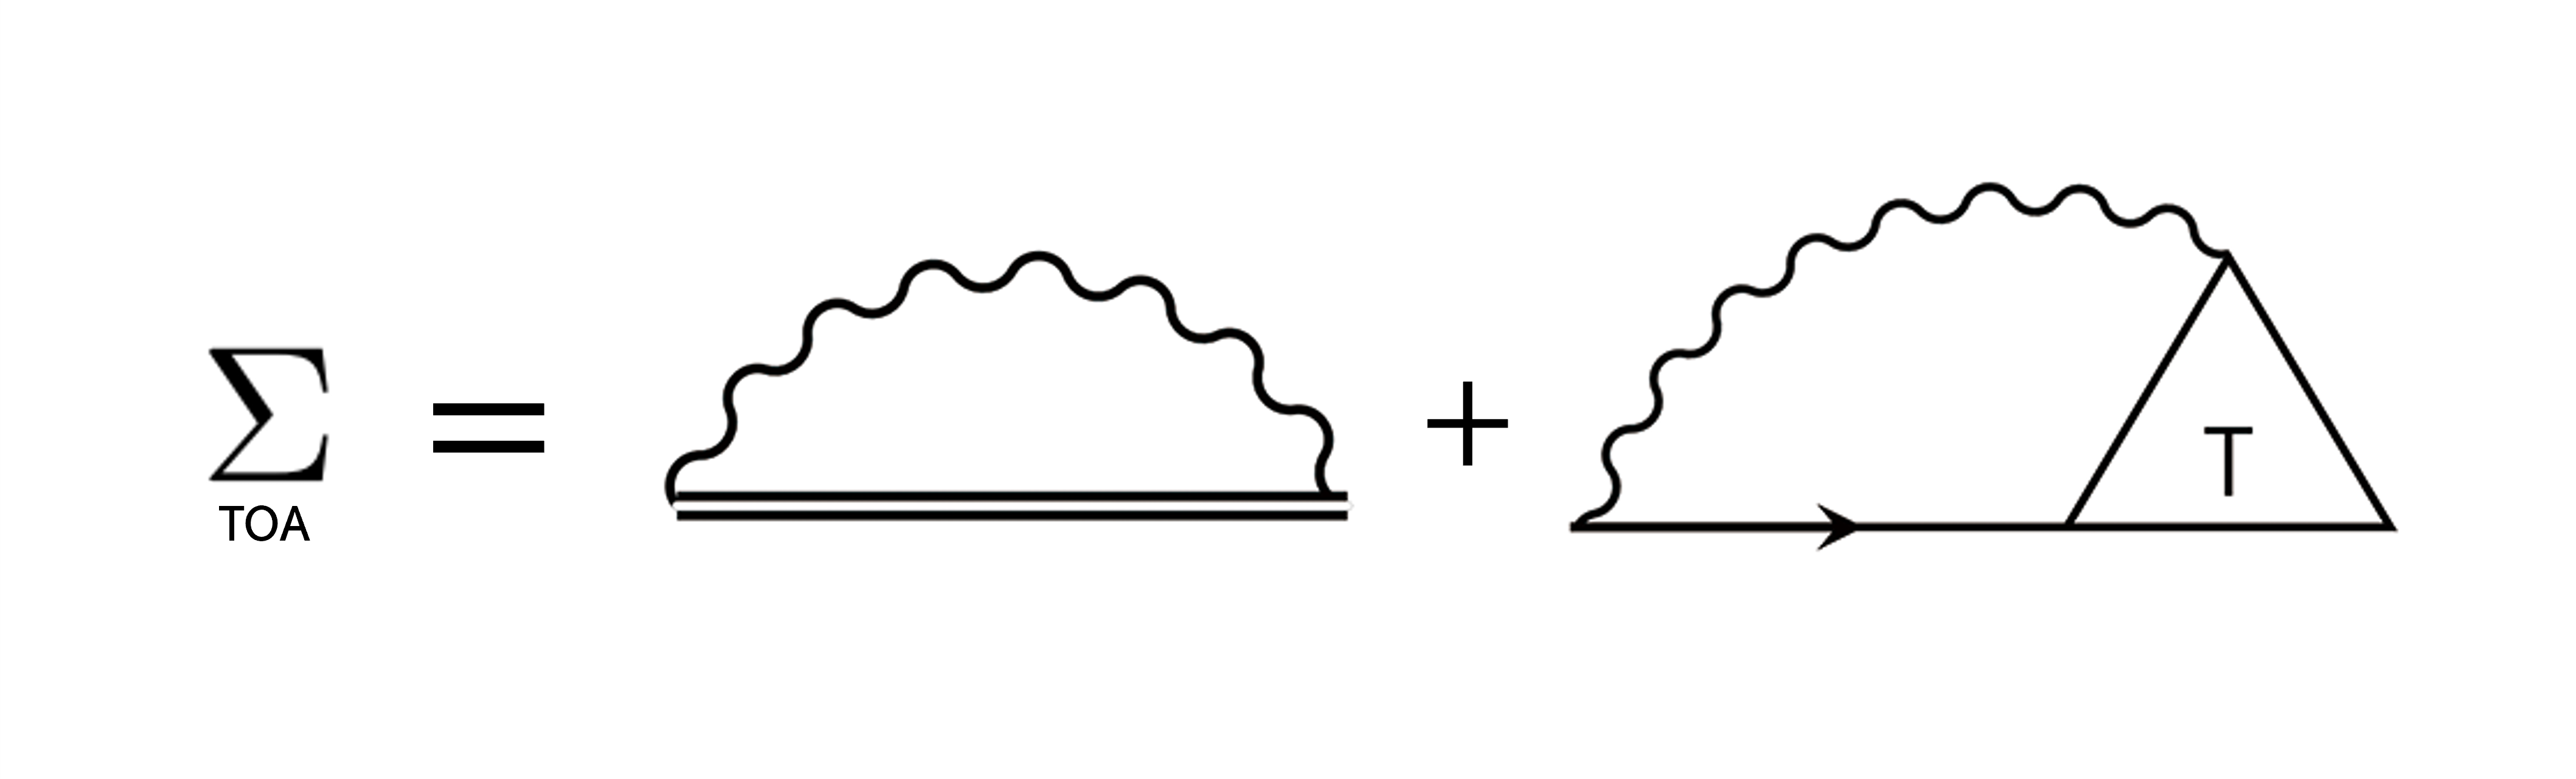
\includegraphics[width=12cm]{TexFigure/TOA_se.png}}
  \centerline{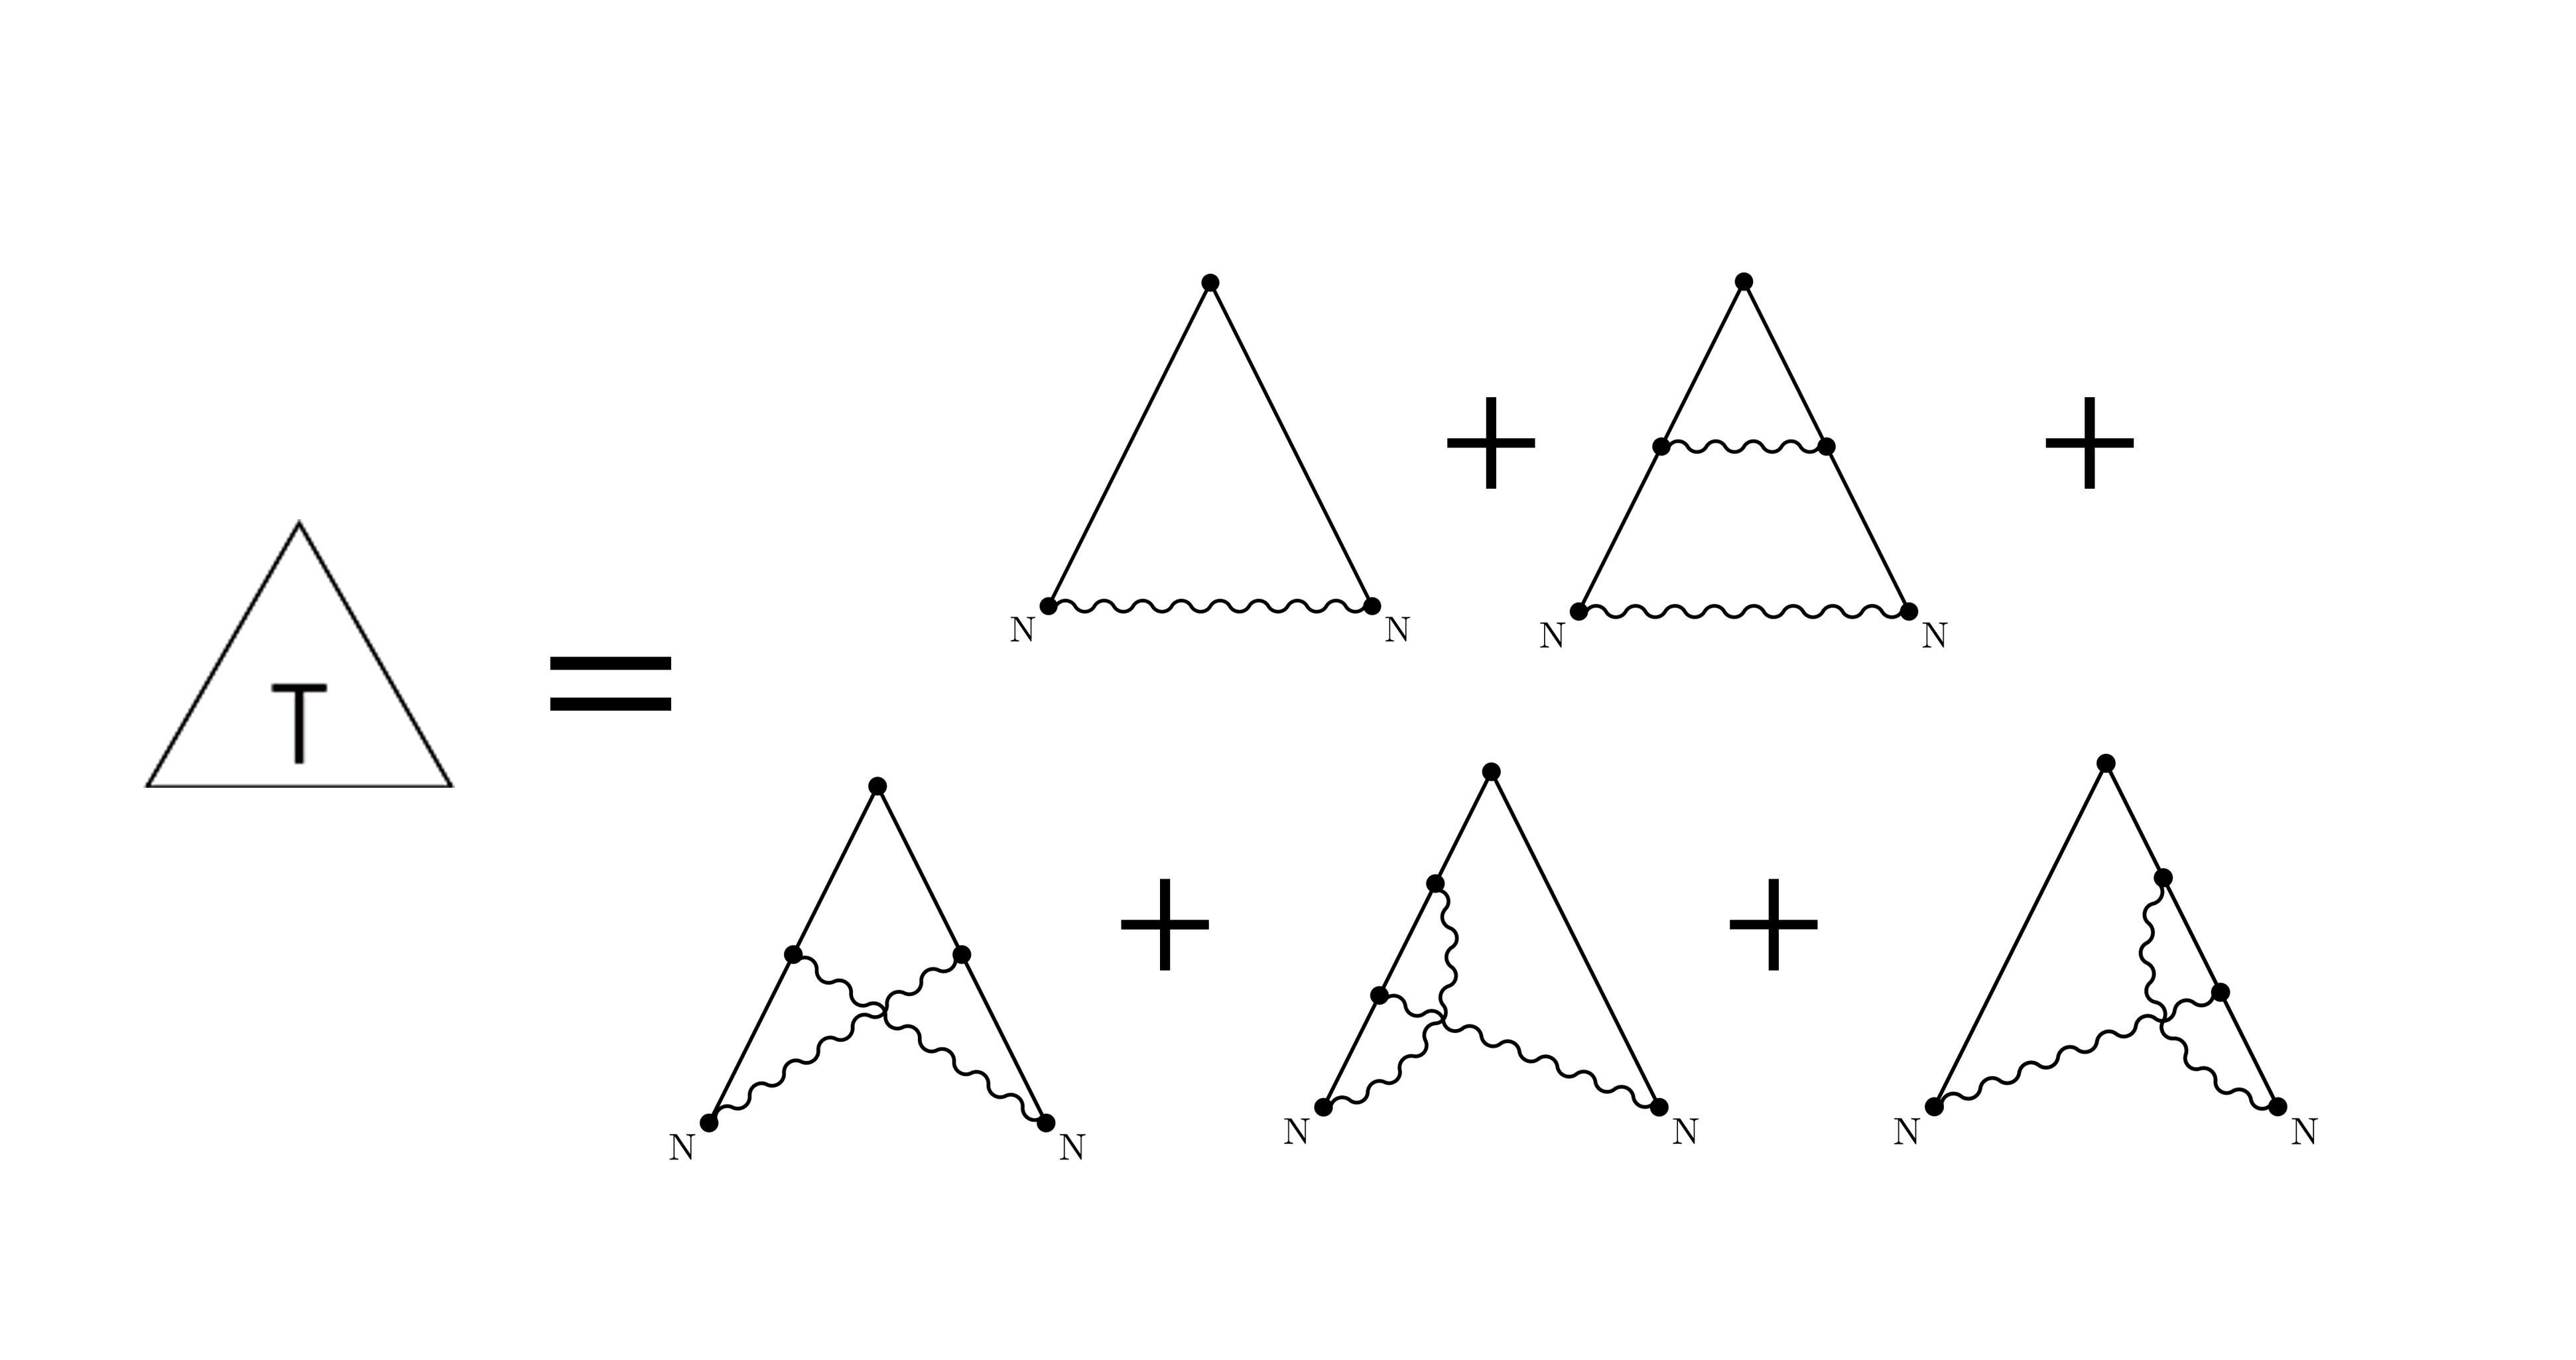
\includegraphics[width=12cm]{TexFigure/TOA_tmat.png}}
  \caption{Self-energy diagram for Five order expansion (TOA). The structure of T matrix was adopted.}
\end{figure}
\end{spacing}
\pagebreak
\end{spacing}
\end{document}
